% !TEX program = xelatex
\documentclass[12pt,a4paper]{ctexart}
\usepackage[left=2.5cm,right=2.5cm,top=2.5cm,bottom=2.5cm,headheight=16pt,headsep=0.55cm,footskip=1.1cm]{geometry}
\usepackage{amsmath}
\usepackage{amssymb}
\usepackage{graphicx}
\usepackage[export]{adjustbox}
\usepackage{xcolor}
\usepackage{booktabs}
\usepackage{tabularx}
\usepackage{longtable}
\usepackage{array}
\usepackage{caption}
\usepackage{fancyhdr}
\usepackage{listings}
\usepackage[section]{placeins}
\usepackage{enumitem}
\usepackage{tocloft}
\usepackage[hidelinks,bookmarks=true,bookmarksnumbered=true,unicode=true]{hyperref}
\usepackage{makecell}

% 双语单元格：中文在上、英文在下，自动按列宽折行（仅用于 p/X 列）
\newcommand{\bip}[2]{\parbox[t]{\linewidth}{\raggedright #1\par\vspace{1.5pt}#2}}

% —— 字体: 西文 Times 系 (TeX Gyre Termes), 代码 DejaVu Sans Mono; 均带回退 ——
\IfFontExistsTF{TeX Gyre Termes}{\setmainfont{TeX Gyre Termes}}{}
\IfFontExistsTF{DejaVu Sans Mono}{\setmonofont{DejaVu Sans Mono}}{%
  \IfFontExistsTF{DejaVuSansMono.ttf}{\setmonofont{DejaVuSansMono.ttf}}{}}

% —— 颜色: 仅保留正文所需的浅灰层级 ——
\definecolor{notegray}{HTML}{595959}
\definecolor{hdrgray}{HTML}{808080}
\definecolor{rulegray}{HTML}{BFBFBF}

% —— 章节样式: 一级标题居中, 二级左对齐; 双语标题第二行用 \normalsize ——
\ctexset{
  section = {format+ = {\heiti\centering}, beforeskip = 20pt plus 4pt minus 2pt, afterskip = 12pt plus 2pt},
  subsection = {format+ = {\heiti}, beforeskip = 14pt plus 3pt minus 2pt, afterskip = 8pt plus 2pt},
}

% —— 图表题注: 双语题注, 表题在上、图题在下, 编号加粗 ——
\captionsetup{font=small, labelfont=bf, labelsep=quad, justification=centering}

% —— 表格列类型 ——
\newcolumntype{Y}{>{\raggedright\arraybackslash}X}
\newcolumntype{L}[1]{>{\raggedright\arraybackslash}p{#1}}

% —— 表格与段落间距 ——
\renewcommand{\arraystretch}{1.12}
\setlength{\tabcolsep}{5pt}
\setlength{\parskip}{4pt plus 1pt minus 1pt}
\setlength{\parindent}{2em}
\setlength{\emergencystretch}{2em}

% —— 列表样式 ——
\setlist[enumerate]{label=（\chinese{enumi}）, leftmargin=2.6em, topsep=4pt, itemsep=2pt, parsep=0pt}
\setlist[itemize]{leftmargin=2em, topsep=4pt, itemsep=2pt, parsep=0pt}

% —— 目录点线 ——
\renewcommand{\cftsecleader}{\cftdotfill{\cftdotsep}}
\renewcommand{\cftsubsecleader}{\cftdotfill{\cftdotsep}}

% —— 页眉页脚 ——
\pagestyle{fancy}
\fancyhf{}
\fancyhead[C]{\footnotesize\color{hdrgray}HUMBUG → IV/DID/RDD · 模拟实验说明文档 · Simulation Documentation}
\fancyfoot[C]{\footnotesize\color{hdrgray}\thepage}
\renewcommand{\headrulewidth}{0.4pt}
\renewcommand{\headrule}{{\color{rulegray}\hrule width\headwidth height 0.4pt}}
\fancypagestyle{frontmatter}{%
  \fancyhf{}%
  \fancyfoot[C]{\footnotesize\color{hdrgray}\thepage}%
  \renewcommand{\headrulewidth}{0pt}}

% —— 代码排版 ——
\lstdefinestyle{pycode}{
  language=Python,
  basicstyle=\ttfamily\fontsize{7.6pt}{9.4pt}\selectfont,
  keywordstyle=\bfseries,
  commentstyle=\color{notegray},
  stringstyle=\color{notegray},
  columns=flexible,
  keepspaces=true,
  breaklines=true,
  breakatwhitespace=true,
  postbreak=\mbox{\textcolor{notegray}{$\hookrightarrow$}\space},
  showstringspaces=false,
  upquote=true,
  xleftmargin=1.2em,
  xrightmargin=1.2em,
  aboveskip=0.5em,
  belowskip=0.9em,
}

\widowpenalty=10000
\clubpenalty=10000

\hypersetup{
  pdftitle={将 HUMBUG 扩展到 IV、DID 与 RDD：模拟实验说明文档 (Extending HUMBUG to IV, DID and RDD)},
  pdfsubject={HUMBUG 批判的因果推断扩展：三组反事实实验与蒙特卡洛模拟},
  pdfkeywords={HUMBUG, 工具变量, 双重差分, 断点回归, 蒙特卡洛, 总量生产函数, 会计恒等式},
}

\begin{document}


% ═══════════ 封面 Cover ═══════════
\begin{titlepage}
\centering
\vspace*{2.4cm}
{\heiti\fontsize{22pt}{32pt}\selectfont 将 HUMBUG 扩展到 IV、DID 与 RDD\par}
\vspace{0.35cm}
{\heiti\fontsize{15pt}{22pt}\selectfont Extending HUMBUG to IV, DID, and RDD\par}
\vspace{1.0cm}
{\heiti\fontsize{13pt}{20pt}\selectfont 工具变量、双重差分与断点回归能否识别资本边际产出\par}
\vspace{0.25cm}
{\heiti\fontsize{11.5pt}{17pt}\selectfont Can IV, DID, and RDD Identify the Marginal Product of Capital?\par}
\vspace{0.25cm}
{\heiti\fontsize{13pt}{20pt}\selectfont ——三组反事实实验与蒙特卡洛模拟说明文档\par}
\vspace{0.25cm}
{\heiti\fontsize{11.5pt}{17pt}\selectfont A Simulation Documentation with Three Counterfactual Experiments and Monte Carlo Evidence\par}
\vspace{1.8cm}
{\rule{\textwidth}{0.4pt}\par}
\vspace{0.6cm}
{\small
\begin{tabular}{@{}l@{\quad}l@{}}
数据给定模式 Data-generating modes： & HUMBUG 字形 / 新古典 / 会计恒等式（\texttt{CONFIG} 切换）\\
识别策略 Identification strategies：   & IV · DID · RDD\\
蒙特卡洛 Monte Carlo：                 & $N = 500$ 次重复 $\times$ 3 种模式\\
文档日期 Date：                        & 2026 年 11 月 1 日 / November 1, 2026\\
\end{tabular}\par}
\vspace{0.6cm}
{\rule{\textwidth}{0.4pt}\par}
\vfill
{\small 模拟实验说明文档 Simulation Documentation\hfill 2026-11-01\par}
\vspace*{0.8cm}
\end{titlepage}


% ═══════════ 目录 TOC ═══════════
\pagenumbering{Roman}
\pagestyle{frontmatter}
\tableofcontents
\clearpage


% ═══════════ 正文 Main body ═══════════
\pagenumbering{arabic}
\pagestyle{fancy}


\section[摘要与核心结论]{摘要与核心结论\\[2pt]\normalsize Summary and Core Findings}

本文档记录一项蒙特卡洛模拟实验的完整过程。实验把 Shaikh（1974）的 HUMBUG 批判扩展到现代因果推断：当 $(\ln(K/L),\ \ln(Y/L))$ 截面数据由矢量字形拼出“HUMBUG”六个字母、从而不存在任何生产函数时，工具变量（IV）、双重差分（DID）与断点回归（RDD）各自识别的是什么参数？给出的“资本边际产出”能否作为新古典理论的证据？

This document records a complete Monte Carlo simulation experiment that extends Shaikh's (1974) HUMBUG critique to modern causal inference. When the cross-sectional data $(\ln(K/L),\ \ln(Y/L))$ are drawn from vector glyphs spelling the six letters of “HUMBUG”—so that no production function exists—what parameter does instrumental variables (IV), difference-in-differences (DID), or regression discontinuity (RDD) actually identify? And can the resulting “marginal product of capital” serve as evidence for neoclassical theory?

实验用 \texttt{CONFIG} 字典切换三种数据给定模式：HUMBUG 字形世界（企业真实边际响应异质）、新古典世界（真实 Cobb-Douglas 生产函数，作为理论为真的校准基准）与会计恒等式世界（$q = w + r\cdot k$，斜率为利润率参数）。三组反事实实验分别在识别假设按构造成立的前提下运行：IV 设干净与脏工具两臂（脏工具经融资成本、市场需求与技术采用渠道直接影响产出，违背排除限制）；DID 构造平行趋势成立的投资补贴面板并辅以安慰剂检验；RDD 构造连续性成立的企业规模门槛。每种方法在三个世界各重复 500 次。

The experiments switch among three data-generating modes via the \texttt{CONFIG} dictionary: a HUMBUG-glyph world (heterogeneous true marginal responses across firms), a neoclassical world (a genuine Cobb-Douglas production function, serving as the calibration benchmark where the theory is true), and an accounting-identity world ($q = w + r\cdot k$, whose slope is the profit-rate parameter). The three counterfactual experiments are each run under identification assumptions that hold by construction: IV is implemented in a clean and a dirty arm (the dirty instrument affects output directly through financing-cost, market-demand, and technology-adoption channels, violating the exclusion restriction); DID constructs an investment-subsidy panel where parallel trends hold and reports a placebo check; RDD constructs a firm-size threshold with continuity holding by construction. Each method is repeated 500 times in each of the three worlds.

核心发现：（1）在 HUMBUG 世界，基准生产函数回归彻底失效（斜率 $-0.005$，$R^2 = 0.001$），但三个“识别成功”的实验给出互相矛盾且均不等于总体平均真实边际产出（$\mu_{\mathrm{pop}} = 0.298$）的答案：2SLS 干净工具约 0.369（识别对象为依从者加权平均 0.367）、脏工具约 0.557（直接渠道按 $1/E[\pi]$ 折入资本系数）、DID 隐含边际产出约 0.498（政策直接效应 $\varphi/\Delta k$ 混入其中）、RDD 局部估计约 0.131（门槛处局部参数，真实值 0.150）。（2）在新古典世界，干净 IV 与 RDD 确实复原了 0.30（覆盖率约 95\%），说明上述失败源于识别对象与理论概念的错位，而非程序错误；脏 IV 与 DID 的偏差则在任何世界都存在，属于识别层面的失败。（3）会计恒等式世界与新古典世界在全部估计量上逐值相同（基准 $R^2$ 甚至等于 1.000），因果识别无法区分“生产函数”与“会计恒等式”两种解释——HUMBUG 批判在因果推断框架下依然成立。

Core findings. (1) In the HUMBUG world, the baseline production-function regression fails completely (slope $-0.005$, $R^2=0.001$), yet the three “successful” identification experiments yield mutually contradictory answers, all differing from the population-average true marginal product ($\mu_{\mathrm{pop}}=0.298$): 2SLS with the clean instrument gives about 0.369 (estimand: complier-weighted average 0.367), the dirty instrument about 0.557 (the direct channel enters the capital coefficient scaled by $1/E[\pi]$), DID implied marginal product about 0.498 (the direct policy effect $\varphi/\Delta k$ is mixed in), and the RDD local estimate about 0.131 (a local parameter at the threshold, true value 0.150). (2) In the neoclassical world, clean IV and RDD do recover 0.30 (coverage about 95\%), showing that the above failures stem from a mismatch between estimand and theoretical concept, not from coding errors; the biases of dirty IV and DID persist in every world and are identification failures proper. (3) The accounting-identity world is numerically identical to the neoclassical world for every estimator (the baseline $R^2$ even equals 1.000), so causal identification cannot distinguish a “production function” from an “accounting identity”—the HUMBUG critique survives within the causal-inference framework.

方法论结论：识别逻辑不等于理论概念。IV、DID、RDD 各自回答的是“特定冲击对特定群体的因果效应”，而新古典理论需要的是“资本作为同质生产要素的边际产出”。统计显著性与识别假设检验均不能弥合这一鸿沟；把前者当作后者的证据，正是本实验所示范的三类陷阱——统计识别失败、因果参数与理论概念之间的解释鸿沟、以及从局部因果效应向一般性经济规律的过度推论。

Methodological conclusion: identification logic is not theoretical concept. IV, DID, and RDD each answer “the causal effect of a particular shock on a particular group,” whereas neoclassical theory wants “the marginal product of capital as a homogeneous factor of production.” Neither statistical significance nor tests of identifying assumptions can bridge this gap; treating the former as evidence for the latter is precisely the three traps this experiment demonstrates—statistical identification failure, the interpretive gap between causal parameter and theoretical concept, and over-extrapolation from local causal effects to general economic laws.

\section[研究背景与方法论立场]{研究背景与方法论立场\\[2pt]\normalsize Background and Methodological Stance}

\subsection[HUMBUG 批判]{HUMBUG 批判\\[1pt]\normalsize The HUMBUG critique}

Shaikh（1974）曾构造了一组在 $(\ln(K/L),\ \ln(Y/L))$ 平面上拼出“HUMBUG”字样的数据，说明只要增加值恒等式（增加值 = 工资总额 + 利润总额，即 $q = w + r\cdot k$）近似成立且要素份额平稳，几乎任何形状的数据都能被 Cobb-Douglas 生产函数良好拟合。Felipe 与 McCombie（2013）在专著中系统重述并强化了这一批评：生产函数回归检验的不是技术关系，而是会计恒等式。剑桥资本争论（Cohen and Harcourt, 2003）从理论侧提出了同构的质疑。

Shaikh (1974) constructed data that trace out the word “HUMBUG” in the $(\ln(K/L),\ \ln(Y/L))$ plane, showing that whenever the value-added identity (value added = wage bill + profit bill, i.e., $q = w + r\cdot k$) holds approximately and factor shares are stationary, almost any shape of data can be fitted well by a Cobb-Douglas production function. Felipe and McCombie (2013) restate and reinforce this critique systematically in their monograph: production-function regressions test, not a technological relation, but an accounting identity. The Cambridge capital controversy (Cohen and Harcourt, 2003) raises a homologous objection from the theoretical side.

对上述批评的一个自然回应是：现代经验研究早已不依赖截面拟合优度，而是依赖准实验识别。本实验要回答的问题是：当数据世界根本不存在生产函数（截面是 HUMBUG 字形）时，三种常见的方法能否识别“资本边际产出”？如果它们在此世界中仍产出精确而显著的“资本系数”，那么该系数是什么？如果不能，失败发生在哪一层——统计识别，还是理论解释？

A natural response to this critique is that modern empirical work no longer relies on cross-sectional goodness of fit but on quasi-experimental identification. The question this experiment asks is: when the data world contains no production function at all (the cross-section is a HUMBUG glyph), can the three common methods identify “the marginal product of capital”? If they still produce a precise and significant “capital coefficient” in that world, what is that coefficient? If they cannot, at which layer does the failure occur—statistical identification, or theoretical interpretation?

\subsection[方法论立场]{方法论立场：不以结果显著论方法失效\\[1pt]\normalsize Methodological stance: significance is not the test of validity}

三种方法的识别逻辑不同，不能简单地把 HUMBUG 数据直接输入三个回归程序、然后以“结果显著”作为方法失效的证据。本实验恰恰相反，要点是让每个方法在自己的识别假设按构造成立的条件下运行：IV 的第一阶段 $F$ 统计量高达数百；DID 的平行趋势由共同时间效应保证、安慰剂检验通过；RDD 的连续性由变量的独立抽取保证。在所有常规诊断全部通过的前提下，再去考察每个估计量到底在估计什么。

The three methods rest on different identification logics, so one cannot simply feed HUMBUG data into three regression programs and treat “a significant result” as evidence that the method has failed. This experiment does the opposite: it is designed so that each method runs under identification assumptions that hold by construction—IV has a first-stage $F$ statistic in the hundreds; DID's parallel trends are guaranteed by common time effects and its placebo test passes; RDD's continuity follows from independent draws of the running variable. With all conventional diagnostics passing, the question becomes what each estimator is actually estimating.

\section[实验设计：CONFIG 与三种数据给定模式]{实验设计：CONFIG 与三种数据给定模式\\[2pt]\normalsize Experimental design: CONFIG and the three data-generating modes}

\subsection[用 CONFIG 切换模式]{用 CONFIG 字典切换数据给定模式\\[1pt]\normalsize Switching data-generating modes with the CONFIG dictionary}

全部实验由脚本顶部的 \texttt{CONFIG} 字典驱动。字段 \texttt{mode} 指定当前数据给定模式，\texttt{modes\_to\_run} 指定批量运行列表，\texttt{focus\_mode} 指定详细图表所用模式；修改这些字段即可在三种数据生成方式之间切换，其余实验与估计代码完全不变。三种模式的定义见表~\ref{tab:modes}。

All experiments are driven by the \texttt{CONFIG} dictionary at the top of the script. The field \texttt{mode} sets the current data-generating mode, \texttt{modes\_to\_run} the batch list, and \texttt{focus\_mode} the mode used for detailed figures; changing these fields switches among the three data-generating regimes while the rest of the experiment and estimation code remains unchanged. The three modes are defined in Table~\ref{tab:modes}.

\begin{table}[htbp]
\centering
\small
\caption{三种数据给定模式\\[1pt]\small Three data-generating modes}\label{tab:modes}
\begin{tabularx}{\textwidth}{l Y Y Y}
\toprule
\makecell[l]{模式\\Mode} & \makecell[l]{基准截面 $(k_0,q_0)$\\Baseline cross-section} & \makecell[l]{真实边际响应 $\mu$\\True marginal response} & \makecell[l]{经济含义\\Economic meaning} \\
\midrule
\texttt{humbug} & \bip{矢量 HUMBUG 字形点（2600 个）}{Vector HUMBUG glyph points (2600)} & \bip{异质：$\alpha+0.20c-0.10s+0.15(s^2-1)+e$}{Heterogeneous} & \bip{不存在生产函数；截面形状任意}{No production function; arbitrary shape} \\
\texttt{neoclassical} & \bip{$k_0\sim N(2.9,0.35)$；$q_0=-0.20+\alpha k_0+\varepsilon$}{Genuine Cobb-Douglas with noise} & \bip{同质：$\mu=\alpha=0.30$}{Homogeneous} & \bip{真实 Cobb-Douglas 世界（校准基准）}{Genuine Cobb-Douglas world (calibration)} \\
\texttt{identity} & \bip{$k_0\sim N(2.9,0.35)$；$q_0=-0.20+\alpha k_0$ 精确成立}{Exact identity, no noise} & \bip{同质：$\mu=\alpha=0.30$}{Homogeneous} & \bip{会计恒等式世界；斜率为利润率参数}{Identity world; slope = profit-rate parameter} \\
\bottomrule
\end{tabularx}
\begin{minipage}{\textwidth}\footnotesize\color{notegray}注 Note：humbug 模式中 $(k_0,q_0)$ 从字形点集随机抽取并加 0.005 的微抖动；$k$、$q$ 分别为对数人均资本与对数人均产出。In the humbug mode, $(k_0,q_0)$ are drawn from the glyph set with 0.005 jitter; $k$ and $q$ are log capital per worker and log output per worker.\par\end{minipage}
\end{table}

\subsection[企业层面的真实结构]{企业层面的真实结构（humbug 模式）\\[1pt]\normalsize The true firm-level structure (humbug mode)}

三种模式的差别只在基准截面与真实响应 $\mu$ 的给定方式。humbug 模式赋予每家企业两个不可由研究者直接观测的特征：信贷约束 $c$ 与企业规模 $s$（相互独立、均服从标准正态，$s$ 截断于 $\pm 3$）。真实边际响应为 $\mu = 0.30 + 0.20c - 0.10s + 0.15(s^2-1) + e$：受信贷约束越强、规模越小的企业边际产出越高，且边际产出随规模呈凸形变化——这为三组实验制造了系统性的异质性与选择性。表~\ref{tab:vars} 汇总全部结构变量与参数。

The three modes differ only in how the baseline cross-section and the true response $\mu$ are specified. In the humbug mode each firm is endowed with two characteristics unobservable to the researcher: a credit constraint $c$ and a firm size $s$ (mutually independent, both standard normal, with $s$ truncated at $\pm 3$). The true marginal response is $\mu = 0.30 + 0.20c - 0.10s + 0.15(s^2-1) + e$: marginal product is higher for firms with tighter credit constraints and smaller size, and varies convexly with size—manufacturing systematic heterogeneity and selection for the three experiments. Table~\ref{tab:vars} summarizes all structural variables and parameters.

\begin{table}[htbp]
\centering
\small
\caption{变量与参数一览\\[1pt]\small Variables and parameters}\label{tab:vars}
\begin{tabularx}{\textwidth}{L{0.25\textwidth} L{0.25\textwidth} Y}
\toprule
\makecell[l]{变量/参数\\Variable / parameter} & \makecell[l]{分布或取值\\Distribution / value} & \makecell[l]{作用\\Role} \\
\midrule
\bip{$c$ 信贷约束（不可观测）}{Credit constraint (unobserved)} & \bip{$N(0,1)$}{Standard normal} & \bip{决定依从强度 $\pi$ 与边际产出 $\mu$}{Determines compliance $\pi$ and marginal product $\mu$} \\
\bip{$s$ 企业规模（可观测）}{Firm size (observed)} & \bip{$N(0,1)$，截断 $\pm 3$}{Truncated at $\pm 3$} & \bip{RDD 门槛变量；DID 处理组遴选（$s<0$）}{RDD running variable; DID treatment selection} \\
\bip{$\mu$ 真实边际产出}{True marginal product} & \bip{$0.30+0.20c-0.10s+0.15(s^2-1)+e$}{$E[\mu]=0.30$} & \bip{资本变化对产出的真实因果响应}{True causal response of output to capital} \\
\bip{$\pi$ 依从强度}{Compliance} & \bip{$0.15+0.55\Phi(0.9c)$}{Positive and monotone} & \bip{第一阶段个体斜率}{First-stage individual slope} \\
\bip{$Z$ 工具变量}{Instrument} & \bip{$N(0,1)$}{Regional credit-supply shock} & \bip{地区信贷供给冲击}{Regional credit-supply shock} \\
\bip{$\delta$ 直接渠道强度}{Direct-channel strength} & \bip{0（干净）/ 0.08（脏）}{0 (clean) / 0.08 (dirty)} & \bip{$Z$ 对 $q$ 的直接影响}{Direct effect of $Z$ on $q$} \\
\bip{$\varphi$ 政策直接效应}{Policy direct effect} & \bip{0.03}{Subsidy direct effect} & \bip{补贴对 $q$ 的直接提升}{Direct subsidy effect on $q$} \\
\bip{$\Delta k$ 补贴资本增量}{Subsidy capital increment} & \bip{0.25}{Design value} & \bip{DID 处理组平均资本跳升}{Average capital jump of treated firms} \\
\bip{$\gamma$ 门槛资本跳升}{Threshold capital jump} & \bip{0.30}{Design value} & \bip{RDD 门槛处资本增量}{Capital increment at the RDD cutoff} \\
\bottomrule
\end{tabularx}
\end{table}

\subsection[三组实验与蒙特卡洛方案]{三组实验与蒙特卡洛方案\\[1pt]\normalsize The three experiments and the Monte Carlo scheme}

实验一（IV）在 800 家企业的截面上比较干净与脏工具两臂；实验二（DID）构造 400 家企业 $\times$ 4 期的面板（前两期为政策前，后两期为政策后）；实验三（RDD）在 1200 家企业的截面上估计规模门槛处的局部效应，并以伪门槛扫描与带宽敏感性考察其可外推性。蒙特卡洛部分对每种模式重复 500 次，每次重新抽取企业与全部冲击，记录每个估计量及其标准误。

Experiment 1 (IV) compares clean and dirty instrument arms on a cross-section of 800 firms; Experiment 2 (DID) constructs a panel of 400 firms $\times$ 4 periods (the first two pre-policy, the last two post-policy); Experiment 3 (RDD) estimates the local effect at a firm-size threshold on a cross-section of 1200 firms, and examines its extrapolability via a pseudo-threshold scan and bandwidth sensitivity. The Monte Carlo component repeats each mode 500 times, redrawing firms and all shocks, and records every estimator and its standard error.

评价采用双重基准：一是相对总体平均真实边际产出 $\mu_{\mathrm{pop}} = E[\mu]$ 的偏差——它代表“新古典理论想要的那个数”；二是相对各方法自身识别对象（概率极限）的偏差——它代表“该方法真正在估计的那个数”。若前者系统偏离而后者收敛，则说明识别成功但概念错位；若两者皆偏，则说明识别层面已经失败。另以 95\% 置信区间对 $\mu_{\mathrm{pop}}$ 的覆盖率衡量“自信地错”的程度。全部汇总见第~\ref{sec:mc} 章。

Evaluation uses a dual benchmark: first, bias relative to the population-average true marginal product $\mu_{\mathrm{pop}}=E[\mu]$—the number “neoclassical theory wants”; second, bias relative to each method's own estimand (probability limit)—the number “the method is actually estimating.” If the former deviates systematically while the latter converges, identification succeeds but the concept is misplaced; if both deviate, identification itself has failed. Coverage of $\mu_{\mathrm{pop}}$ by 95\% confidence intervals measures the degree of “confident error.” All summaries are given in Chapter~\ref{sec:mc}.

\section[HUMBUG 数据生成与基准回归]{HUMBUG 数据生成与基准回归\\[2pt]\normalsize HUMBUG data generation and baseline regression}

\subsection[矢量字形生成]{矢量字形生成（HUMBUG 函数）\\[1pt]\normalsize Vector-glyph generation (the HUMBUG function)}

字形数据按矢量方式生成，由脚本中的 \texttt{HUMBUG()} 函数实现：用 matplotlib 的 \texttt{TextPath} 把衬线粗体“HUMBUG”渲染为字形轮廓多边形，沿每段轮廓的弧长均匀采样共 2600 个点，再线性归一化到 $(k, q)$ 平面——$k \in [2.05,\ 3.90]$，$q \in [0.60,\ 0.82]$。与栅格化再取点的方式相比，矢量采样不依赖分辨率，点沿笔画均匀分布，且完全可复现。图~\ref{fig:baseline} 左侧面板即生成的字形截面。

The glyph data are generated as vectors by the \texttt{HUMBUG()} function in the script: matplotlib's \texttt{TextPath} renders the serif bold word “HUMBUG” as glyph-outline polygons, points are sampled uniformly along the arc length of each contour up to a total of 2600, and the result is linearly normalized into the $(k,q)$ plane—$k\in[2.05,3.90]$, $q\in[0.60,0.82]$. Compared with rasterizing and then sampling, vector sampling is resolution-independent, distributes points evenly along strokes, and is fully reproducible. The left panel of Figure~\ref{fig:baseline} shows the resulting glyph cross-section.

\subsection[三种模式的基准 OLS]{三种模式的基准 OLS 结果\\[1pt]\normalsize Baseline OLS in the three modes}

研究者面对任何数据的第一步通常是估计截面生产函数：

A researcher's first step with any data is usually to estimate a cross-sectional production function:

\begin{equation}\label{eq:baseline}
q_i = \beta_0 + \beta_1 k_i + \varepsilon_i .
\end{equation}

三种模式下的结果见表~\ref{tab:baseline} 与图~\ref{fig:baseline}。

Results across the three modes are in Table~\ref{tab:baseline} and Figure~\ref{fig:baseline}.

\begin{table}[htbp]
\centering
\small
\caption{基准 OLS 回归（无政策、无工具的原始截面）\\[1pt]\small Baseline OLS (raw cross-section, no policy, no instrument)}\label{tab:baseline}
\begin{tabularx}{\textwidth}{l r r r Y}
\toprule
\makecell[l]{模式\\Mode} & \makecell[c]{斜率 $\hat{\beta}$\\Slope} & \makecell[c]{标准误\\SE} & $R^2$ & \makecell[l]{解读\\Interpretation} \\
\midrule
HUMBUG 字形 & $-0.0051$ & 0.0041 & 0.0013 & \bip{竖直笔画摧毁拟合，无函数关系}{Vertical strokes destroy the fit; no functional relation} \\
新古典世界 & 0.2999 & 0.0008 & 0.9916 & \bip{真生产函数，正常复原}{Genuine production function; recovered} \\
会计恒等式 & 0.3000 & $\approx 0$ & 1.0000 & \bip{恒等式精确成立}{Exact identity; $R^2=1.000$} \\
\bottomrule
\end{tabularx}
\begin{minipage}{\textwidth}\footnotesize\color{notegray}注 Note：样本量 $n=1200$。恒等式模式的标准误数量级为 $10^{-16}$，回归残差由浮点误差构成。Sample size $n=1200$. In the identity mode the SE is of order $10^{-16}$; residuals are floating-point error.\par\end{minipage}
\end{table}

\begin{figure}[htbp]
\centering
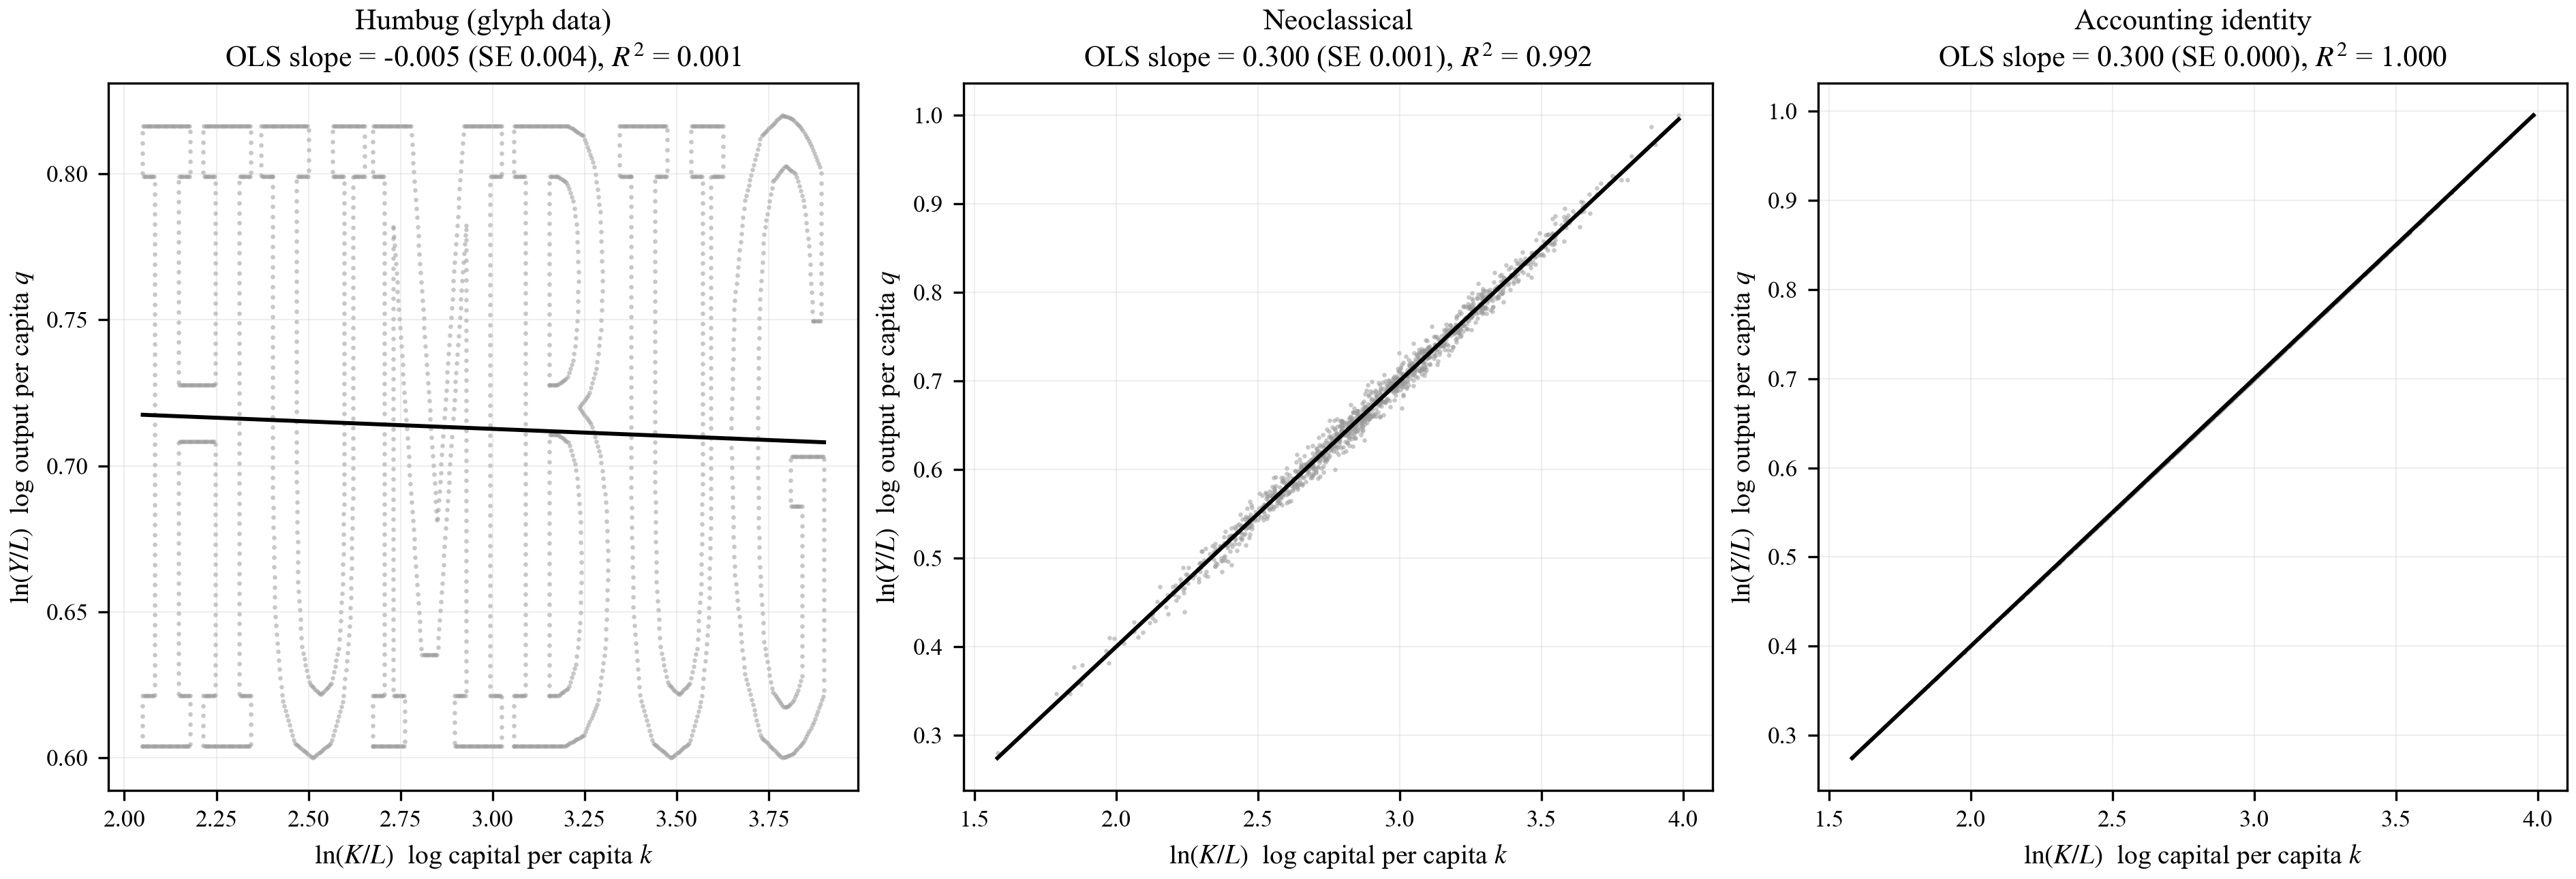
\includegraphics[width=\textwidth]{fig1_baseline.png}
\caption{三种数据给定模式的基准截面与 OLS 拟合\\[1pt]\small Baseline cross-sections and OLS fits in the three data-generating modes}\label{fig:baseline}
\end{figure}

两点观察：
\begin{enumerate}
  \item HUMBUG 字形的竖直笔画使 $E[q|k]$ 近似为常数，OLS 斜率与零无异，$R^2$ 仅 0.0013——这正是字形世界“没有生产函数”的直观含义；字母沿水平方向排布，横竖笔画之间不存在可拟合的函数关系，资本在这里甚至不是可排序的同质要素。
  \item 恒等式世界的 $R^2 = 1.000$ 高于真生产函数世界的 0.9916：拟合更好不等于更接近真理，恒等式世界的数据由定义式精确生成，反而比带噪声的真实技术关系“更干净”。
\end{enumerate}
这两点共同构成后文所有实验的背景：截面回归既可能一无所获（字形世界），也可能完美命中一个并非生产函数的规律（恒等式世界）。

Two observations. (i) The vertical strokes of the glyph make $E[q\mid k]$ approximately constant; the OLS slope is indistinguishable from zero and $R^2$ is only 0.0013—the intuitive meaning of “no production function” in the glyph world. Letters are arranged horizontally, with no fittable functional relation between horizontal and vertical strokes; capital here is not even a rankable homogeneous factor. (ii) The identity world has $R^2=1.000$, higher than the genuine production-function world's 0.9916: a better fit does not mean closer to truth; the identity data are generated exactly by a definitional formula and are therefore “cleaner” than a noisy genuine technological relation. Together, these two observations form the backdrop for all subsequent experiments: cross-sectional regression may yield nothing (glyph world) or may perfectly hit a regularity that is not a production function (identity world).

\section[实验一：工具变量]{实验一：工具变量能否识别资本边际产出\\[2pt]\normalsize Experiment 1: Can IV identify the marginal product of capital?}

\subsection[设计]{设计：干净与脏工具两臂\\[1pt]\normalsize Design: clean and dirty instrument arms}

设定工具变量 $Z$ 为地区信贷供给冲击（$N(0,1)$），其应当显著影响企业资本投入。数据生成由 \texttt{iv\_simulate()} 与 \texttt{iv\_estimate()} 两个函数完成：第一阶段中企业依从强度 $\pi = 0.15 + 0.55\Phi(0.9c)$ 随信贷约束单调递增且恒为正（满足单调性与正向依从），资本与产出方程为：

Let the instrument $Z$ be a regional credit-supply shock ($N(0,1)$), which should significantly affect firms' capital input. Data generation is handled by the functions \texttt{iv\_simulate()} and \texttt{iv\_estimate()}: in the first stage each firm's compliance $\pi=0.15+0.55\Phi(0.9c)$ rises monotonically with the credit constraint and is always positive (satisfying monotonicity and positive compliance); the capital and output equations are:

\begin{equation}\label{eq:iv}
k_i = k_{0i} + \pi_i Z_i + v_i, \qquad
q_i = q_{0i} + \mu_i \Delta k_i + \delta Z_i + e_i .
\end{equation}

两臂共享同一组冲击 $(Z, v, e)$，唯一的差别是 $\delta$：干净工具臂 $\delta = 0$，$Z$ 影响产出的唯一渠道是资本，排除限制满足；脏工具臂 $\delta = 0.08$，$Z$ 同时经融资成本、市场需求与技术采用渠道直接影响产出，排除限制被违背——这正对应现实中“信贷冲击影响投资、但也直接影响企业其他生产条件”的典型担忧。恰好识别的 2SLS 等价于 Wald 比率，其概率极限为：

Both arms share the same shocks $(Z,v,e)$; the only difference is $\delta$: in the clean arm $\delta=0$, the sole channel from $Z$ to output is capital, so the exclusion restriction holds; in the dirty arm $\delta=0.08$, $Z$ also affects output directly through financing-cost, market-demand, and technology-adoption channels, violating exclusion—precisely the standard concern that “a credit shock affects investment but also directly affects other production conditions.” The just-identified 2SLS equals the Wald ratio, whose probability limit is:

\begin{equation}\label{eq:ivplim}
\operatorname{plim} \hat{\beta}_{IV}(\delta) = \frac{E[\mu\pi] + \delta}{E[\pi]} .
\end{equation}

干净臂识别依从者加权平均 $E[\mu\pi]/E[\pi]$——即 Imbens-Angrist（1994）的局部平均处理效应（LATE）型参数；脏工具把直接渠道按 $1/E[\pi]$ 折算进资本系数。两面都不是总体平均 $\mu_{\mathrm{pop}}$——这是因果参数与理论概念之间的解释鸿沟的解析形式。

The clean arm identifies the complier-weighted average $E[\mu\pi]/E[\pi]$—the local average treatment effect (LATE)-type parameter of Imbens and Angrist (1994); the dirty instrument folds the direct channel into the capital coefficient via $1/E[\pi]$. Neither equals the population average $\mu_{\mathrm{pop}}$—the analytic form of the interpretive gap between causal parameter and theoretical concept.

\subsection[结果]{结果\\[1pt]\normalsize Results}

\begin{table}[htbp]
\centering
\small
\caption{IV 实验结果（HUMBUG 世界，代表性单次抽样）\\[1pt]\small IV results (HUMBUG world, representative single draw)}\label{tab:iv}
\begin{tabularx}{\textwidth}{L{0.25\textwidth} r r c r r}
\toprule
\makecell[l]{估计量\\Estimator} & \makecell[c]{估计值\\Estimate} & \makecell[c]{标准误\\SE} & \makecell[c]{95\% 置信区间\\95\% CI} & \makecell[c]{识别对象\\Estimand} & $\mu_{\mathrm{pop}}$ \\
\midrule
\bip{OLS（实验样本）}{OLS (experiment sample)} & 0.165 & 0.011 & [0.144, 0.186] & — & 0.304 \\
\bip{\textbf{2SLS 干净工具（$\delta=0$）}}{\textbf{2SLS clean instrument ($\delta=0$)}} & \textbf{0.344} & \textbf{0.023} & [0.298, 0.389] & 0.373 & 0.304 \\
\bip{\textbf{2SLS 脏工具（$\delta=0.08$）}}{\textbf{2SLS dirty instrument ($\delta=0.08$)}} & \textbf{0.526} & \textbf{0.028} & [0.471, 0.581] & 0.561 & 0.304 \\
\bottomrule
\end{tabularx}
\begin{minipage}{\textwidth}\footnotesize\color{notegray}注 Note：$\mu_{\mathrm{pop}}$ 为 IV 子样本（$n=800$）均值 0.304；与第 9 节 RDD 样本 0.303、MC 均值 0.298 的差异来自子样本构成。第一阶段 $\hat{\pi}=0.439$（SE 0.019），$F=545$，远超常用临界值 10；MC 中最差一次 $F=308$。识别对象：干净臂 $E[\mu\pi]/E[\pi]=0.373$，脏臂 $(E[\mu\pi]+\delta)/E[\pi]=0.561$。The $\mu_{\mathrm{pop}}$ column is the IV subsample mean (0.304); differences from the RDD subsample (0.303) and MC mean (0.298) reflect subsample composition. First stage: $\hat\pi=0.439$ (SE 0.019), $F=545$, far above 10; worst case in MC: $F=308$.\par\end{minipage}
\end{table}

\begin{figure}[htbp]
\centering
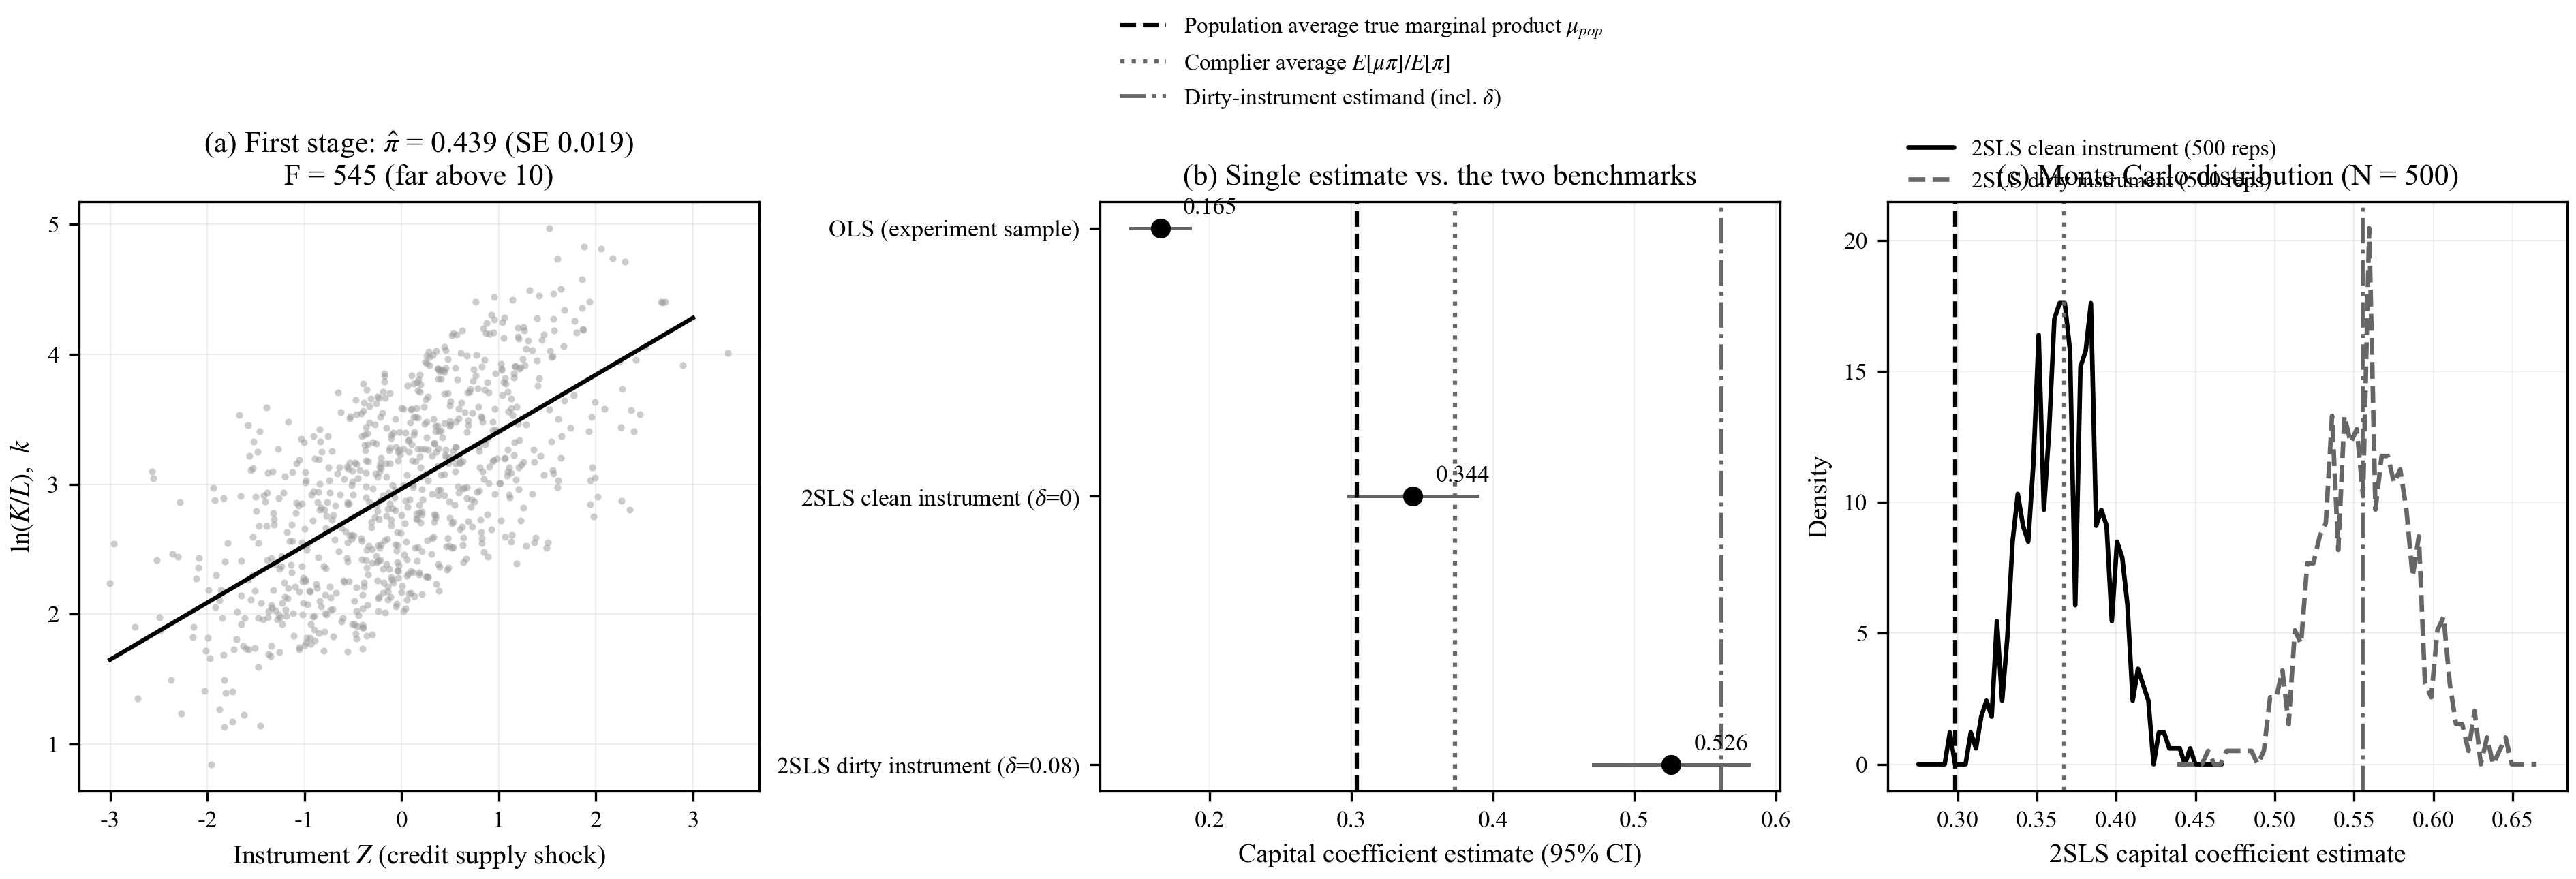
\includegraphics[width=\textwidth]{fig2_iv.png}
\caption{IV 实验：第一阶段、单次估计与蒙特卡洛分布\\[1pt]\small IV experiment: first stage, single estimate, and Monte Carlo distribution}\label{fig:iv}
\end{figure}

\subsection[解读]{解读：识别成功与解释鸿沟\\[1pt]\normalsize Interpretation: identification success and the interpretive gap}

第一，干净工具臂展示了“识别成功但概念错位”。估计值 0.344（500 次蒙特卡洛均值 0.369）紧贴其识别对象——依从者加权平均 0.367，而与总体平均 $\mu_{\mathrm{pop}} = 0.298$ 系统偏离：依从者是信贷约束更强、边际产出更高的企业，工具变量识别的是这批企业的局部平均因果效应。对 $\mu_{\mathrm{pop}}$ 的置信区间覆盖率仅 19.0\%——估计量精确而自信地指向了另一个参数。即使完全接受计量经济学的识别条件（排除限制、单调性、独立性），也不能自动得到新古典理论所需要的“全体企业的资本边际产出”。

First, the clean arm exhibits “identification success with conceptual mismatch.” The estimate 0.344 (MC mean over 500 draws 0.369) is close to its estimand—the complier-weighted average 0.367—but systematically far from the population mean $\mu_{\mathrm{pop}}=0.298$: compliers are firms with tighter credit constraints and higher marginal products, and IV identifies the local average causal effect for this group. The 95\% CI covers $\mu_{\mathrm{pop}}$ only 19.0\% of the time—the estimator points precisely and confidently at another parameter. Even if all econometric identifying conditions (exclusion, monotonicity, independence) are fully accepted, one does not automatically obtain “the marginal product of capital for all firms” that neoclassical theory requires.

第二，脏工具臂展示了识别层面的失败如何被强第一阶段掩盖。$F$ 高达 545、系数在 1\% 水平高度显著，但估计值 0.526 混入了 $\delta/E[\pi] \approx 0.19$ 的直接渠道贡献：第二阶段估计出来的资本系数已经不是资本边际产出，而是“单位资本变动所承载的全部 $Z$ 效应”。研究者若只报告第一阶段强度与第二阶段显著性，将毫无察觉。

Second, the dirty arm shows how identification failure can be masked by a strong first stage. $F$ reaches 545 and the coefficient is highly significant at 1\%, but the estimate 0.526 includes a direct-channel contribution $\delta/E[\pi]\approx 0.19$: the second-stage capital coefficient is no longer the marginal product of capital but “the total $Z$ effect carried by a unit change in capital.” A researcher reporting only first-stage strength and second-stage significance would remain unaware.

第三，作为校准，新古典世界（理论为真、$\mu$ 同质）中干净工具的估计为 0.299、500 次覆盖率 95.0\%——方法本身没有问题。对照之下，HUMBUG 世界的偏离不是程序错误，而是识别对象与理论概念的错位；脏工具的偏差则在两个世界同样存在（新古典世界均值 0.488），属于可归因于设计的识别失败。

Third, as a calibration, in the neoclassical world (where the theory is true and $\mu$ is homogeneous) the clean instrument estimates 0.299 with 95.0\% coverage over 500 draws—the method itself is fine. By contrast, the HUMBUG-world deviation is not a coding error but a mismatch between estimand and theoretical concept; the dirty-instrument bias, in contrast, appears in both worlds (neoclassical mean 0.488) and is an identification failure attributable to design.

\section[实验二：DID]{实验二：DID 的政策处理效应不等于资本边际产出\\[2pt]\normalsize Experiment 2: DID policy effects are not the marginal product of capital}

\subsection[设计]{设计：投资补贴面板与平行趋势的构造性成立\\[1pt]\normalsize Design: subsidy panel with parallel trends by construction}

政策设定为面向小企业（$s < 0$，占比约 48.5\%）的投资补贴。面板由 \texttt{did\_simulate()} 生成（400 家企业 $\times$ 4 期，第 3 期起为政策后），企业层面方程为：

The policy is an investment subsidy for small firms ($s<0$, about 48.5\% of the sample). The panel is generated by \texttt{did\_simulate()} (400 firms $\times$ 4 periods, with the third period onward post-policy); the firm-level equation is:

\begin{equation}\label{eq:did}
q_{it} = \eta_i + \tau_t + \mu_i \Delta k_{it} + \varphi D_{it} + u_{it} .
\end{equation}

平行趋势由共同时间效应 $\tau_t$ 按构造保证；政策通过两条路径影响产出：补贴诱发的资本增量 $\Delta k = 0.25$（经真实边际响应 $\mu$ 折算）与直接效应 $\varphi = 0.03$——后者汇总了政策同时改变企业融资约束、技术选择与市场竞争地位的三条渠道。研究者通常的做法是先估计政策总效应 ATT，再除以资本的平均实际增量 $\Delta K$ 得到“隐含资本边际产出”，或者直接跑带企业与时间固定效应的生产函数回归。两者由 \texttt{did\_estimate()} 与 \texttt{did\_placebo()} 实现。

Parallel trends are guaranteed by construction through common time effects $\tau_t$. The policy affects output through two paths: a subsidy-induced capital increment $\Delta k=0.25$ (scaled by the true marginal response $\mu$) and a direct effect $\varphi=0.03$—the latter aggregating three channels through which the policy simultaneously changes financing constraints, technology choice, and competitive position. The standard practice is to estimate the overall ATT and then divide by the average realized capital increment $\Delta K$ to obtain an “implied marginal product,” or to run a firm-and-time fixed-effects production-function regression. Both are implemented in \texttt{did\_estimate()} and \texttt{did\_placebo()}.

\subsection[结果]{结果\\[1pt]\normalsize Results}

\begin{table}[htbp]
\centering
\small
\caption{DID 实验结果（HUMBUG 世界，代表性单次抽样）\\[1pt]\small DID results (HUMBUG world, representative single draw)}\label{tab:did}
\begin{tabularx}{\textwidth}{L{0.27\textwidth} r r c Y}
\toprule
\makecell[l]{估计量\\Estimator} & \makecell[c]{估计值\\Estimate} & \makecell[c]{标准误\\SE} & \makecell[c]{95\% 置信区间\\95\% CI} & \makecell[l]{真实构成 / 基准\\True composition / benchmark} \\
\midrule
\bip{安慰剂前置趋势}{Placebo pre-trend} & 0.0001 & 0.0029 & $[-0.006, 0.006]$ & \bip{应接近 0（前趋势平行）}{Should be near 0 (parallel pre-trends)} \\
\bip{\textbf{DID 政策效应 ATT $\hat{\theta}$}}{\textbf{DID policy effect ATT $\hat{\theta}$}} & \textbf{0.1274} & \textbf{0.0038} & [0.120, 0.135] & \bip{$E[\mu|\text{处理组}]\cdot\Delta k+\varphi$}{$=0.3752\times 0.25+0.03$} \\
\bip{资本 DID 增量 $\Delta K$}{DID capital increment $\Delta K$} & 0.2507 & — & — & \bip{设计值 0.25}{Design value 0.25} \\
\bip{\textbf{隐含边际产出 $\hat{\theta}/\Delta K$}}{\textbf{Implied marginal product $\hat{\theta}/\Delta K$}} & \textbf{0.508} & \textbf{0.015} & [0.478, 0.538] & \bip{识别对象 $E[\mu|\text{处理组}]+\varphi/\Delta k$}{Estimand $=0.495$} \\
\bip{FE 生产回归 $\hat{\beta}$}{FE production regression $\hat{\beta}$} & 0.503 & 0.014 & [0.474, 0.531] & \bip{与隐含边际产出同一识别对象}{Same estimand as implied MPK} \\
\bip{基准：$\mu_{\mathrm{pop}}$ / 处理组 $\bar{\mu}$}{Benchmarks: $\mu_{\mathrm{pop}}$ / treated $\bar{\mu}$} & 0.292 & — & — & \bip{DID 子样本平均 / 处理组真实平均}{Subsample mean / treated mean $=0.375$} \\
\bottomrule
\end{tabularx}
\begin{minipage}{\textwidth}\footnotesize\color{notegray}注 Note：安慰剂检验把第 2 期当伪政策期，500 次蒙特卡洛中均值 $-0.0001$、覆盖 0 的比例 94.6\%，检验水平正确；隐含边际产出的蒙特卡洛均值为 0.498。The placebo treats period 2 as a pseudo-policy date; across 500 MC draws the mean is $-0.0001$ and the share covering 0 is 94.6\%, indicating correct level; the MC mean of implied MPK is 0.498.\par\end{minipage}
\end{table}

\begin{figure}[htbp]
\centering
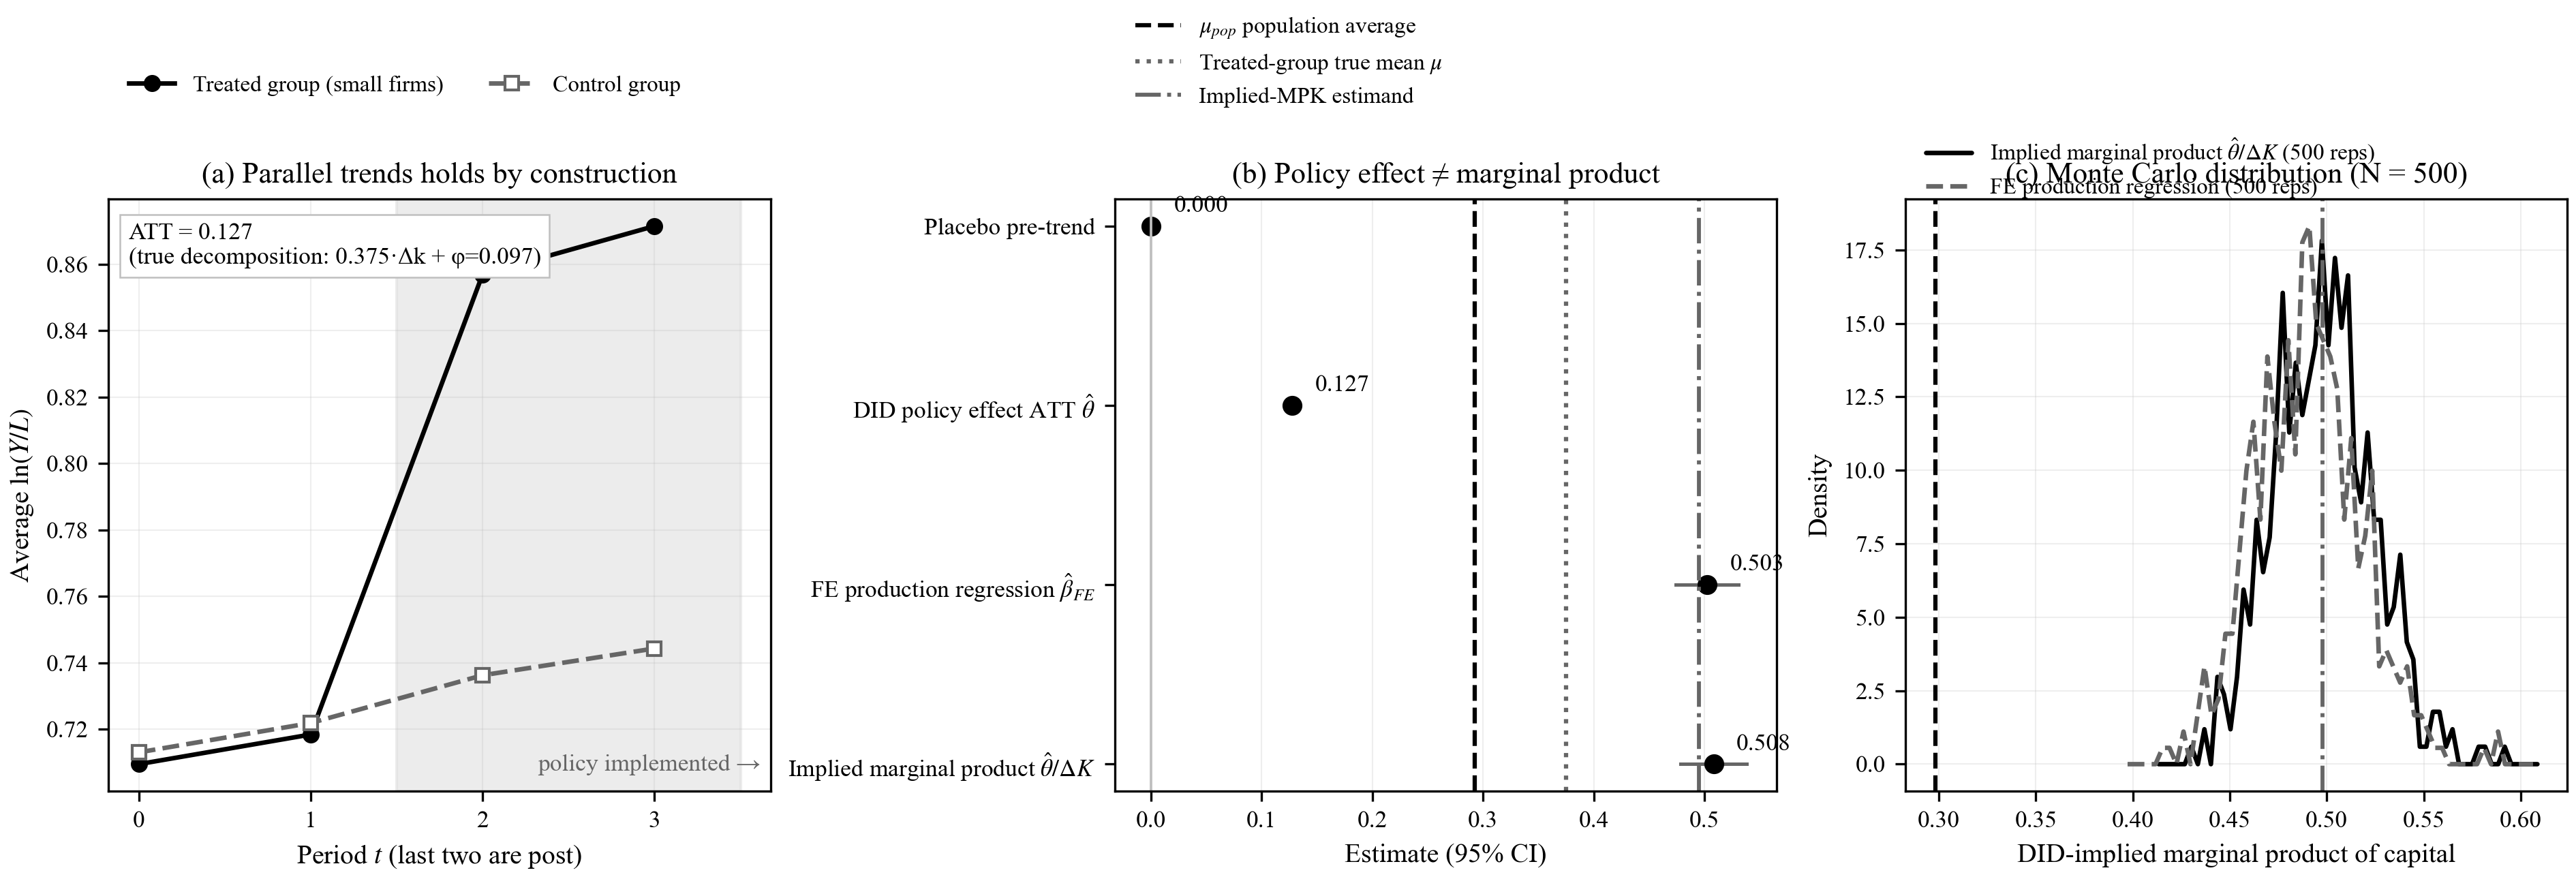
\includegraphics[width=\textwidth]{fig3_did.png}
\caption{DID 实验：平行趋势、估计森林与蒙特卡洛分布\\[1pt]\small DID experiment: parallel trends, estimator forest, and Monte Carlo distribution}\label{fig:did}
\end{figure}

\subsection[解读]{解读：政策因果效应不等于生产技术\\[1pt]\normalsize Interpretation: a policy causal effect is not a production technology}

DID 正确地识别了它该识别的：政策总效应 ATT = 0.1274，在抽样误差范围内覆盖其真实构成（0.1274 对 0.1238，差约 1 个标准误）。问题出在外推这一步：把 ATT 除以 $\Delta K$ 得到隐含边际产出 0.508，与 DID 子样本平均 $\mu_{\mathrm{pop}} = 0.292$ 相去甚远。偏差来自两个可分解的来源：其一，处理组是小企业，其真实平均边际产出 0.375 本身高于总体平均（选择性与资本边际回报异质性）；其二，$\varphi/\Delta k = 0.120$ 的直接渠道贡献被整体记到了资本头上。即便平行趋势成立、安慰剂检验通过，这一混合依然无法由 DID 自身分离。

DID correctly identifies what it should: the overall ATT is 0.1274, covering its true composition within sampling error (0.1274 vs.\ 0.1238, about one standard error apart). The problem arises in the extrapolation step: dividing ATT by $\Delta K$ yields an implied marginal product of 0.508, far from the DID subsample mean $\mu_{\mathrm{pop}}=0.292$. The bias has two decomposable sources: first, the treated group consists of small firms whose true average marginal product of 0.375 is itself above the population mean (selection plus heterogeneity in marginal returns to capital); second, the direct-channel contribution $\varphi/\Delta k=0.120$ is attributed entirely to capital. Even with parallel trends holding and the placebo passing, DID by itself cannot separate this mixture.

更值得注意的是 FE 生产回归：它与 DID 隐含边际产出给出几乎相同的数值（0.503 对 0.508）。两条常规程序互相印证，但印证的是同一个错误——资本在政策期恰好是处理指示变量的线性函数，任何只用政策期资本变异的估计量都识别同一个混合参数。程序之间的一致性不等于概念的正确性。DID 可以识别资本政策的因果效应，却不能仅凭这一结果识别资本本身的生产技术属性。

More striking is the FE production regression: it yields virtually the same value as the DID implied marginal product (0.503 vs.\ 0.508). The two routine procedures corroborate each other—but they corroborate the same error: during the policy period capital is exactly a linear function of the treatment indicator, so any estimator that uses only policy-period capital variation identifies the same mixture. Agreement among procedures is not conceptual validity. DID can identify the causal effect of a capital policy; by itself it cannot identify the technological properties of capital.

\section[实验三：RDD]{实验三：RDD 局部因果效应与一般性生产规律\\[2pt]\normalsize Experiment 3: RDD local causal effects vs.\ general production laws}

\subsection[设计]{设计：规模门槛与连续性的构造性成立\\[1pt]\normalsize Design: size threshold with continuity by construction}

政策按企业规模设置补贴门槛：规模不低于 $s^* = 0$ 的企业获得投资补贴，资本在门槛处跳升 $\gamma = 0.3$。数据由 \texttt{rdd\_simulate()} 生成：

The policy sets a subsidy threshold on firm size: firms with $s\ge s^*=0$ receive an investment subsidy, and capital jumps by $\gamma=0.3$ at the threshold. Data are generated by \texttt{rdd\_simulate()}:

\begin{equation}\label{eq:rdd}
D_i = \mathbf{1}\{s_i \ge s^*\}, \qquad
k_i = k_{0i} + \gamma D_i + w_i, \qquad
q_i = q_{0i} + \mu_i(\gamma D_i + w_i) + e_i .
\end{equation}

所有潜变量 $(k_0, q_0, \mu)$ 与 $s$ 独立抽取，条件期望在门槛处连续——连续性假设按构造成立，且本设计不含政策的直接效应（$\gamma$ 之外的渠道为零），RDD 在其识别范围内完全干净。研究者用两侧局部线性拟合估计资本跳跃 $J_k$ 与产出跳跃 $J_q$，其比值（等价于以 $D$ 为工具的局部 2SLS，由 \texttt{rdd\_estimate()} 实现）的极限为门槛附近的局部平均边际产出 $E[\mu\,|\,s = s^*]$。为考察该估计的局部性，\texttt{rdd\_pseudo\_scan()} 进一步把政策门槛反事实地平移到 $s^* \in \{-2, -1.5, \ldots, +2\}$ 并重复估计。

All latent variables $(k_0,q_0,\mu)$ are drawn independently of $s$, so conditional expectations are continuous at the threshold—continuity holds by construction, and the design contains no direct policy effect (channels other than $\gamma$ are zero), making RDD completely clean within its identification scope. The researcher estimates the capital jump $J_k$ and the output jump $J_q$ by local linear fits on both sides; their ratio (equivalent to a local 2SLS using $D$ as an instrument, implemented in \texttt{rdd\_estimate()}) converges to the local average marginal product near the threshold, $E[\mu\mid s=s^*]$. To probe the local nature of this estimate, \texttt{rdd\_pseudo\_scan()} counterfactually shifts the policy threshold to $s^*\in\{-2,-1.5,\ldots,+2\}$ and repeats the estimate.

\subsection[结果]{结果\\[1pt]\normalsize Results}

\begin{table}[htbp]
\centering
\small
\caption{RDD 实验结果（HUMBUG 世界，代表性单次抽样）\\[1pt]\small RDD results (HUMBUG world, representative single draw)}\label{tab:rdd}
\begin{tabularx}{\textwidth}{L{0.33\textwidth} c Y}
\toprule
\makecell[l]{指标\\Metric} & \makecell[c]{数值\\Value} & \makecell[l]{说明\\Note} \\
\midrule
\bip{资本跳跃 $J_k$}{Capital jump $J_k$} & 0.402 & \bip{门槛两侧局部线性拟合的截距差；设计值 $\gamma=0.3$，单次受 $w$ 噪声影响偏离设计值，MC 均值接近 0.3}{Intercept difference between local-linear fits; design value $\gamma=0.3$; single draws deviate due to $w$ noise; MC mean near 0.3} \\
\bip{产出跳跃 $J_q$}{Output jump $J_q$} & 0.043 & \bip{约等于 $\gamma\cdot E[\mu|s\approx 0]$}{Approximately $\gamma\cdot E[\mu\mid s\approx 0]$} \\
\bip{\textbf{RDD 局部估计 $\hat{\beta}$（$h=1.0$）}}{\textbf{RDD local estimate $\hat{\beta}$ ($h=1.0$)}} & \textbf{0.106（SE 0.036）} & \bip{95\% CI [0.036, 0.176]；局部真值 $E[\mu|s{=}0]=0.150$}{95\% CI [0.036, 0.176]; local true value $0.150$} \\
\bip{带宽敏感性 $h=0.5/1.5/2.0$}{Bandwidth sensitivity $h=0.5/1.5/2.0$} & 0.157 / 0.116 / 0.079 & \bip{MC 均值 0.155 / 0.104 / 0.079}{MC means 0.155 / 0.104 / 0.079} \\
\bip{伪门槛扫描（$s^*$ 从 $-2$ 到 $+2$）}{Pseudo-threshold scan ($s^*$ from $-2$ to $+2$)} & 0.680 $\to$ 0.106 $\to$ 0.695 & \bip{估计值随门槛移动，描出异质性曲线（图~\ref{fig:rdd}c）}{The estimate moves with the threshold, tracing the heterogeneity curve (Figure~\ref{fig:rdd}c)} \\
\bip{外推检验}{Extrapolation check} & 0.032 vs.\ 0.091 & \bip{全体企业资本同增 $\gamma$ 时，低估 65\%}{Under-estimates by 65\% when all firms' capital rises by $\gamma$} \\
\bip{基准 $\mu_{\mathrm{pop}}$}{Benchmark $\mu_{\mathrm{pop}}$} & 0.303 & \bip{RDD 子样本的平均真实边际产出}{Mean true MPK of the RDD subsample} \\
\bottomrule
\end{tabularx}
\end{table}

\begin{figure}[htbp]
\centering
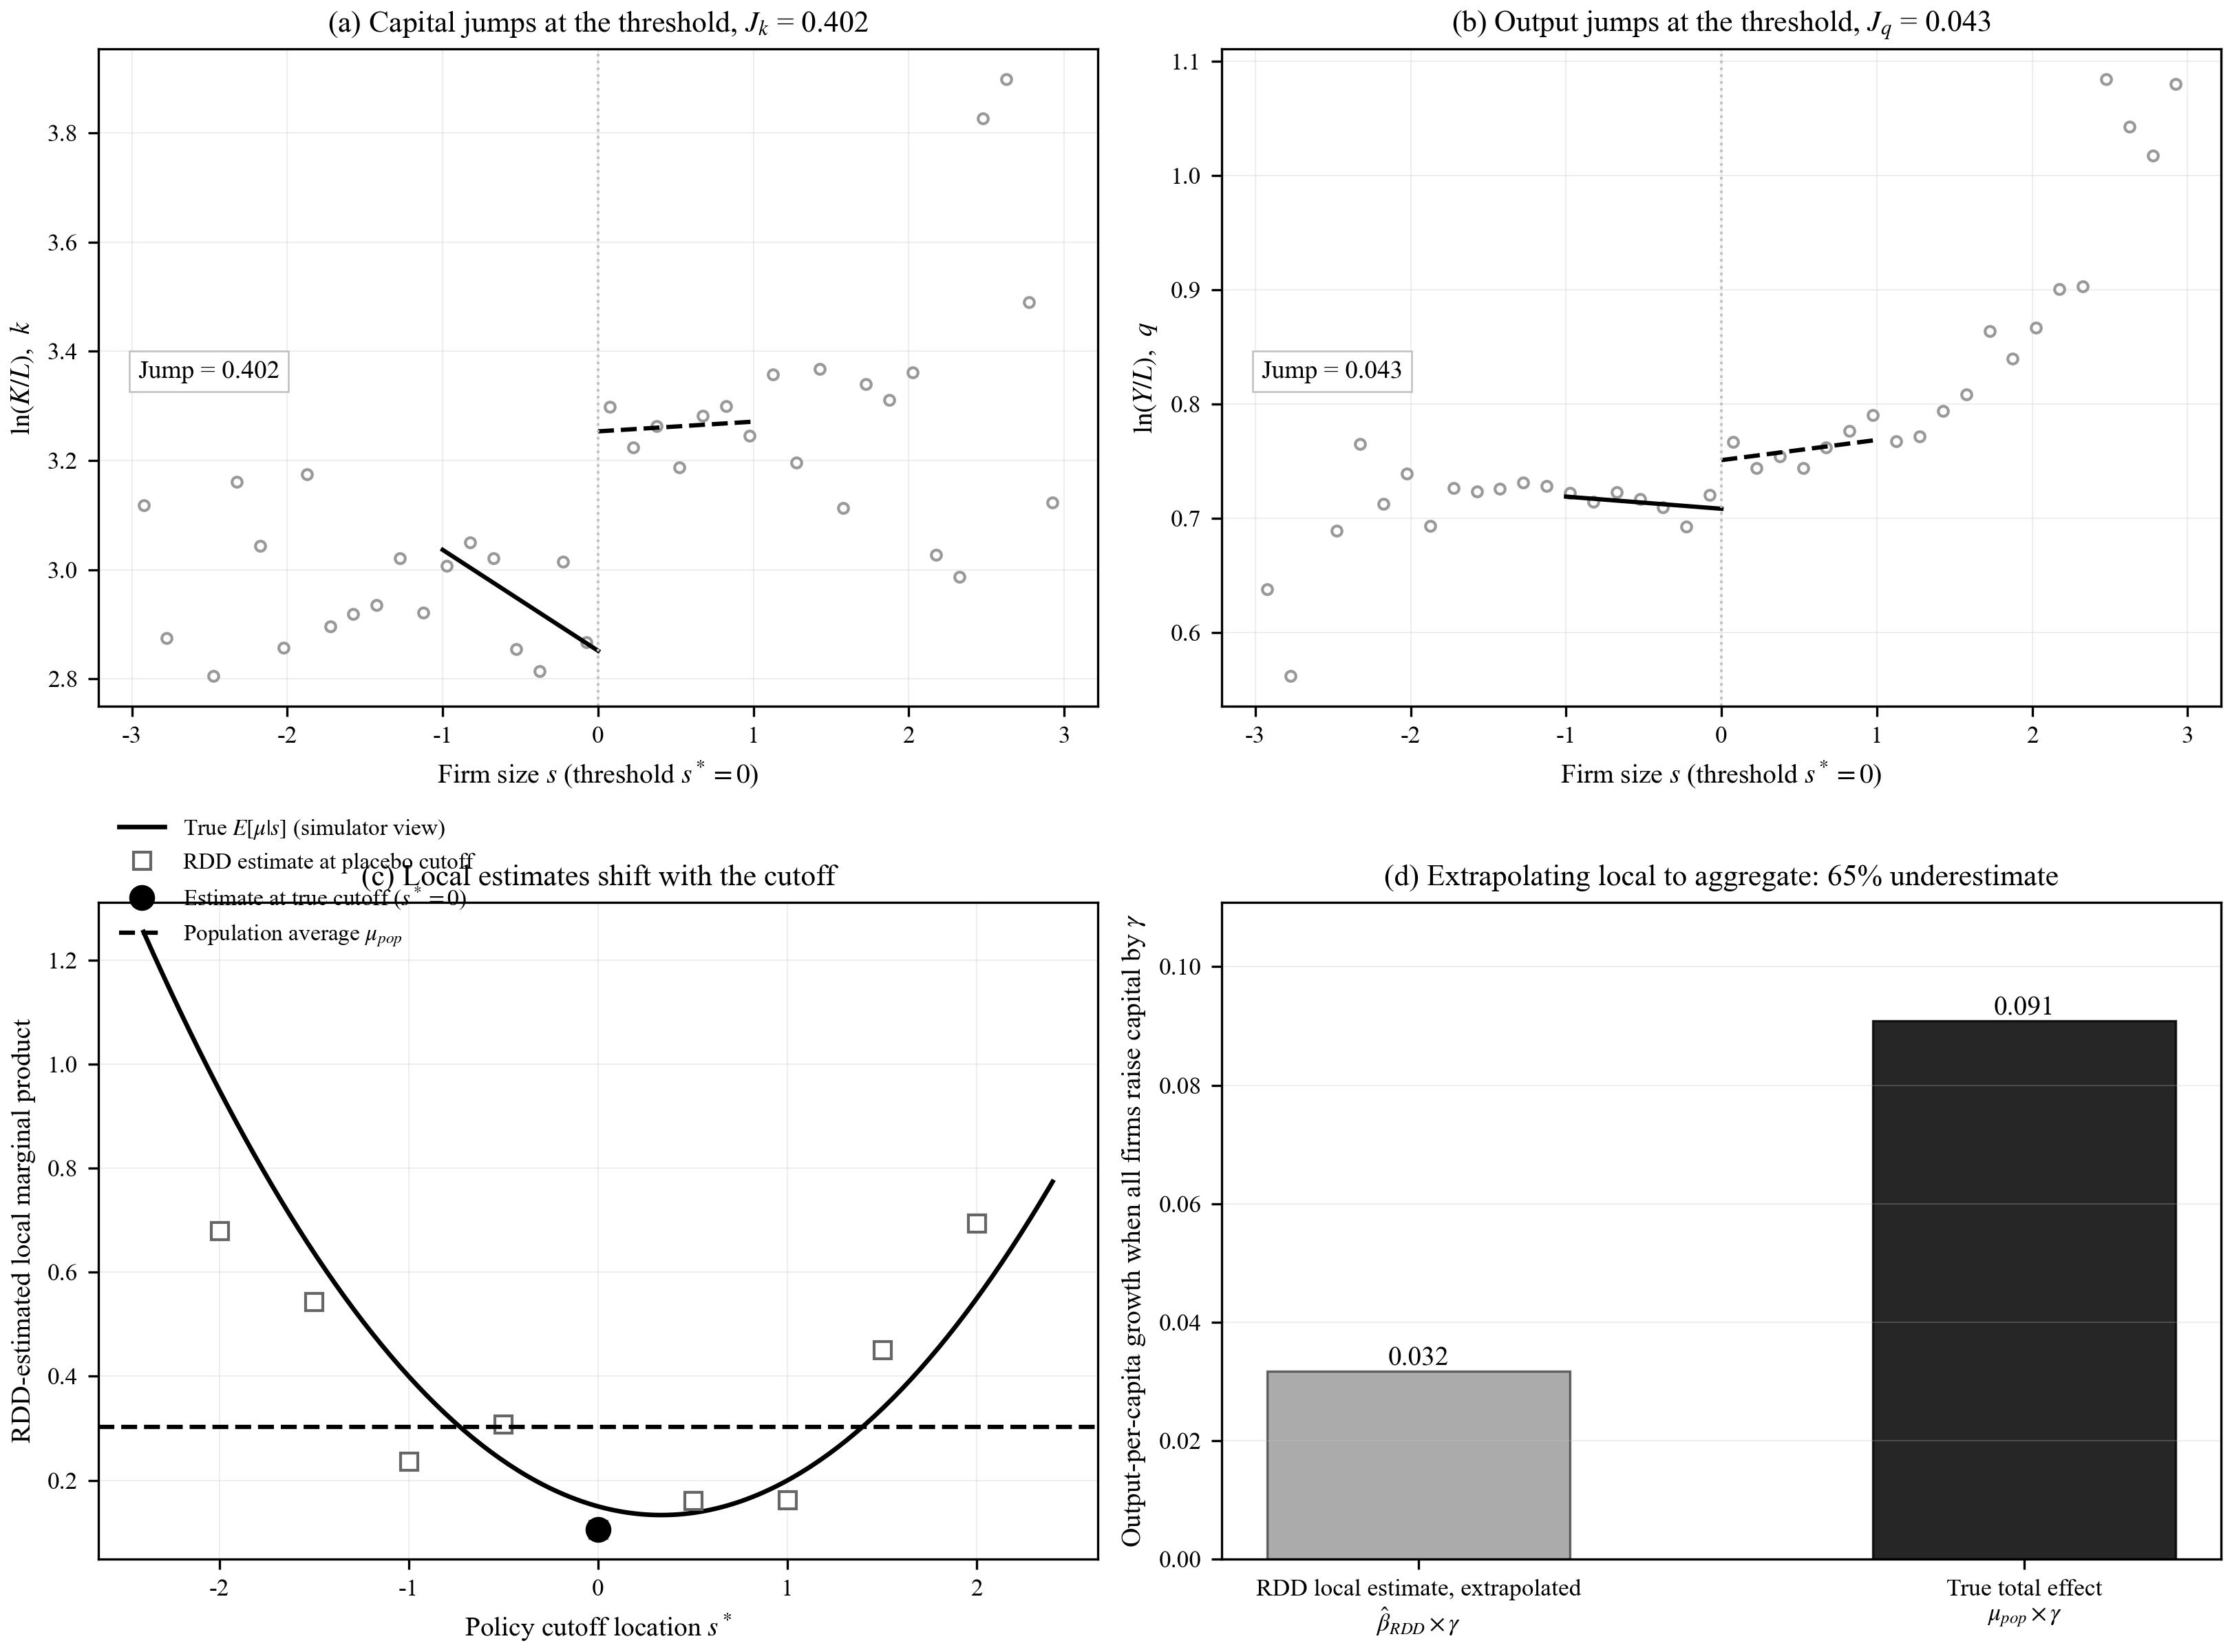
\includegraphics[width=0.86\textwidth]{fig4_rdd.png}
\caption{RDD 实验：门槛跳跃、异质性扫描与外推误差\\[1pt]\small RDD experiment: threshold jump, heterogeneity scan, and extrapolation error}\label{fig:rdd}
\end{figure}

\subsection[解读]{解读：从局部到一般的过度推论\\[1pt]\normalsize Interpretation: over-extrapolation from local to general}

RDD 估计 0.106（蒙特卡洛均值 0.131）忠实地落在门槛处的局部真值 0.150 附近，且显著不为零——统计识别没有失败。问题在于这个数字回答的问题极其具体：“规模恰好位于门槛附近的企业、因补贴而增加一单位资本的产出响应”。本设计中 $E[\mu|s]$ 呈 U 形（$0.30 - 0.10s + 0.15(s^2-1)$），门槛恰在低谷附近，于是局部估计系统性低于总体平均 0.298；伪门槛扫描显示，把门槛移到 $s^* = \pm 2$，同一个程序立刻给出 0.680 与 0.695——估计的是门槛位置的函数，不是资本的属性。

The RDD estimate 0.106 (MC mean 0.131) falls faithfully near the local true value 0.150 at the threshold and is significantly nonzero—statistical identification has not failed. The problem is that the number answers a very specific question: “the output response to a one-unit capital increase induced by the subsidy for firms whose size happens to be near the threshold.” In this design $E[\mu\mid s]$ is U-shaped ($0.30-0.10s+0.15(s^2-1)$), and the threshold happens to sit near the trough, so the local estimate is systematically below the population mean 0.298; the pseudo-threshold scan shows that shifting the threshold to $s^*=\pm 2$ makes the same procedure deliver 0.680 and 0.695 immediately—the estimate is a function of the threshold location, not an attribute of capital.

由此，RDD 的结果不能证明三件新古典解释所需的事：不能证明所有企业具有相同的资本边际产出（异质性恰恰是结论的一部分）；不能证明资本可以作为同质生产要素加总——在 HUMBUG 世界，$(k, q)$ 截面甚至不构成函数关系，加总无从谈起；更不能证明总量生产函数具备理论所要求的性质。若研究者把局部估计外推为一般生产规律，用以预测“全体企业资本同增 $\gamma$”的总效应，将得到 0.032 而非真实的 0.091，低估约 65\%（蒙特卡洛均值口径：0.131 对 0.298，低估约 56\%）。RDD 的问题不一定是统计识别失败，而可能是从局部因果效应向一般性经济规律的过度推论。

Thus RDD's results cannot establish the three things the neoclassical interpretation requires: it cannot show that all firms share the same marginal product of capital (heterogeneity is precisely part of the conclusion); it cannot show that capital aggregates as a homogeneous factor of production—in the HUMBUG world the $(k,q)$ cross-section does not even constitute a functional relation, so aggregation is moot; and it certainly cannot show that the aggregate production function has the properties theory requires. If a researcher extrapolates the local estimate as a general production law to predict the total effect of “all firms' capital rising by $\gamma$,” the result is 0.032 instead of the true 0.091, an under-estimate of about 65\% (MC mean: 0.131 vs.\ 0.298, about 56\%). The RDD problem is not necessarily statistical identification failure but possibly over-extrapolation from local causal effects to general economic laws.

\section[蒙特卡洛汇总]{蒙特卡洛汇总（$N = 500$）与三个世界的对照\\[2pt]\normalsize Monte Carlo summary ($N=500$) and the three-world comparison}\label{sec:mc}

\subsection[汇总结果]{汇总结果\\[1pt]\normalsize Summary results}

\begingroup\scriptsize
\setlength{\tabcolsep}{3.5pt}
\begin{longtable}{L{0.10\textwidth}L{0.21\textwidth}rrrrc}
\caption{蒙特卡洛汇总：各方法 $\times$ 各模式（500 次重复）\\[1pt]\small Monte Carlo summary: methods $\times$ modes (500 repetitions)}\label{tab:mc}\\
\toprule
\makecell[l]{模式\\Mode} & \makecell[l]{估计量\\Estimator} & \makecell[c]{均值\\Mean} & \makecell[c]{SD\\SD} & \makecell[c]{偏差 vs $\mu_{\mathrm{pop}}$\\Bias vs $\mu_{\mathrm{pop}}$} & \makecell[c]{偏差 vs 识别对象\\Bias vs estimand} & \makecell[c]{95\%CI 覆盖\\Coverage} \\
\midrule
\endfirsthead
\multicolumn{7}{l}{\footnotesize\color{notegray}（续表 Continued Table~\ref{tab:mc}）}\\
\toprule
\makecell[l]{模式\\Mode} & \makecell[l]{估计量\\Estimator} & \makecell[c]{均值\\Mean} & \makecell[c]{SD\\SD} & \makecell[c]{偏差 vs $\mu_{\mathrm{pop}}$\\Bias vs $\mu_{\mathrm{pop}}$} & \makecell[c]{偏差 vs 识别对象\\Bias vs estimand} & \makecell[c]{95\%CI 覆盖\\Coverage} \\
\midrule
\endhead
\endfoot
\bottomrule
\endlastfoot
HUMBUG & \bip{\textbf{$\mu_{\mathrm{pop}}$（基准）}}{\textbf{$\mu_{\mathrm{pop}}$ (baseline)}} & 0.2984 & — & — & — & — \\
HUMBUG & \bip{基准 OLS}{Baseline OLS} & $-0.0001$ & 0.0041 & $-0.2984$ & $-0.2984$ & 0.0\% \\
HUMBUG & \bip{2SLS 干净}{2SLS clean} & 0.3685 & 0.0254 & 0.0702 & 0.0014 & 19.0\% \\
HUMBUG & \bip{2SLS 脏}{2SLS dirty} & 0.5571 & 0.0303 & 0.2587 & 0.0016 & 0.0\% \\
HUMBUG & \bip{DID 隐含 MPK}{DID implied MPK} & 0.4983 & 0.0257 & 0.2000 & 0.0004 & 0.0\% \\
HUMBUG & \bip{FE 回归}{FE regression} & 0.4901 & 0.0269 & 0.1917 & $-0.0079$ & 0.0\% \\
HUMBUG & \bip{RDD 局部}{RDD local} & 0.1305 & 0.0545 & $-0.1678$ & $-0.0195$ & 19.6\% \\
\addlinespace
Neoclassical & \bip{\textbf{$\mu_{\mathrm{pop}}$（基准）}}{\textbf{$\mu_{\mathrm{pop}}$ (baseline)}} & 0.3000 & — & — & — & — \\
Neoclassical & \bip{基准 OLS}{Baseline OLS} & 0.3000 & 0.0008 & $-0.0000$ & $-0.0000$ & 95.2\% \\
Neoclassical & \bip{2SLS 干净}{2SLS clean} & 0.3000 & 0.0019 & 0.0000 & 0.0000 & 95.0\% \\
Neoclassical & \bip{2SLS 脏}{2SLS dirty} & 0.4883 & 0.0071 & 0.1883 & 0.0001 & 0.0\% \\
Neoclassical & \bip{DID 隐含 MPK}{DID implied MPK} & 0.4199 & 0.0076 & 0.1199 & $-0.0001$ & 0.0\% \\
Neoclassical & \bip{FE 回归}{FE regression} & 0.4113 & 0.0075 & 0.1113 & $-0.0087$ & 0.0\% \\
Neoclassical & \bip{RDD 局部}{RDD local} & 0.3001 & 0.0106 & 0.0001 & 0.0001 & 95.8\% \\
\addlinespace
Identity & \bip{\textbf{$\mu_{\mathrm{pop}}$（基准）}}{\textbf{$\mu_{\mathrm{pop}}$ (baseline)}} & 0.3000 & — & — & — & — \\
Identity & \bip{基准 OLS}{Baseline OLS} & 0.3000 & 0.0000 & $-0.0000$ & $-0.0000$ & 0.2\% \\
Identity & \bip{2SLS 干净}{2SLS clean} & 0.3000 & 0.0017 & 0.0000 & 0.0000 & 94.6\% \\
Identity & \bip{2SLS 脏}{2SLS dirty} & 0.4881 & 0.0070 & 0.1881 & $-0.0001$ & 0.0\% \\
Identity & \bip{DID 隐含 MPK}{DID implied MPK} & 0.4205 & 0.0081 & 0.1205 & 0.0005 & 0.0\% \\
Identity & \bip{FE 回归}{FE regression} & 0.4116 & 0.0078 & 0.1116 & $-0.0084$ & 0.0\% \\
Identity & \bip{RDD 局部}{RDD local} & 0.3003 & 0.0091 & 0.0003 & 0.0003 & 96.2\% \\
\addlinespace
\end{longtable}
\endgroup

\begin{minipage}{\textwidth}\footnotesize\color{notegray}注 Note：“偏差 vs 识别对象”为估计量均值减去其概率极限（模拟器视角计算）。覆盖率低于 95\% 表示该方法置信区间系统性地不包含总体平均真实边际产出。DID 隐含 MPK 的标准误按 $\delta$ 方法（$\mathrm{SE}(\theta)\slash\Delta K$）近似。“Bias vs.\ estimand” is the mean estimate minus its probability limit (computed from the simulator's perspective). Coverage below 95\% means the method's CI systematically excludes the population-average true marginal product. DID implied MPK's SE is approximated by the delta method.\par\end{minipage}

\begin{figure}[htbp]
\centering
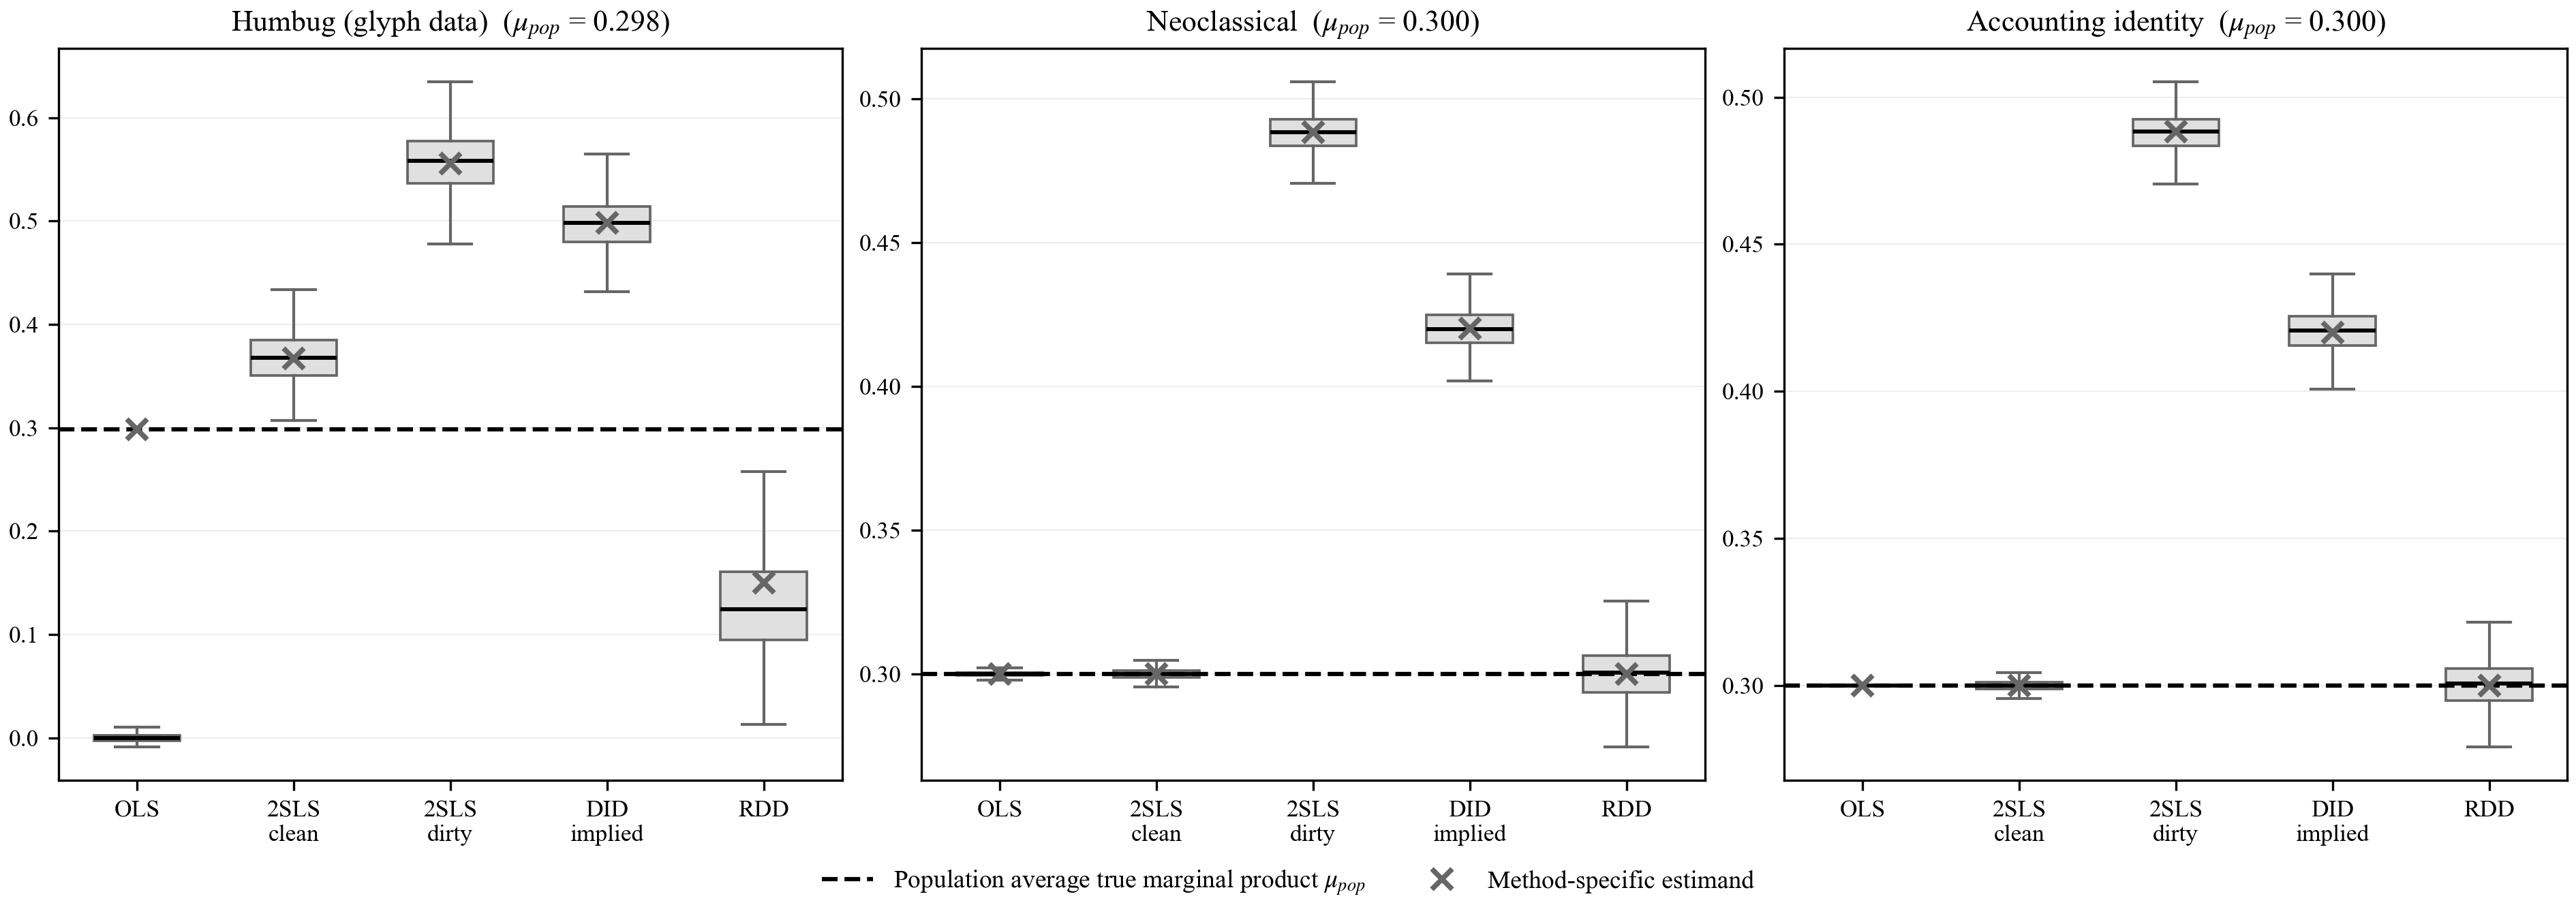
\includegraphics[width=\textwidth]{fig5_mc.png}
\caption{蒙特卡洛分布汇总：三个世界 $\times$ 五种估计量\\[1pt]\small Monte Carlo distributions: three worlds $\times$ five estimators}\label{fig:mc}
\end{figure}

\subsection[三个世界的对照]{三个世界的对照：校准与不可区分性\\[1pt]\normalsize Comparing the three worlds: calibration and indistinguishability}

表~\ref{tab:mc} 与图~\ref{fig:mc} 给出三层对照。第一层（HUMBUG 字形世界）：全部方法相对各自识别对象的偏差都在 0.01 以内——识别是成功的；相对 $\mu_{\mathrm{pop}}$ 的偏差则系统性非零，覆盖率从 19.0\%（干净 IV）到 19.6\%（RDD）不等，基准 OLS 与 DID 隐含 MPK 同样远离。估计量们精确、显著、自信，却各自指向不同的参数。

Table~\ref{tab:mc} and Figure~\ref{fig:mc} give a three-layer comparison. First layer (HUMBUG-glyph world): every method's bias relative to its own estimand is within 0.01—identification succeeds; but bias relative to $\mu_{\mathrm{pop}}$ is systematically nonzero, with coverage ranging from 19.0\% (clean IV) to 19.6\% (RDD), and baseline OLS and DID implied MPK equally far off. The estimators are precise, significant, and confident—yet each points at a different parameter.

第二层（新古典世界）：干净 IV 与 RDD 的覆盖率分别为 95.0\% 与 95.8\%，均值皆为 0.300——在理论为真的世界里方法工作正常，这为 HUMBUG 世界的失败提供了归因依据：脏 IV（偏差 0.188）与 DID 隐含 MPK（偏差 0.120）的失败源于设计中的排除限制违背与直接渠道，在任何世界都无法消除；而干净 IV 与 RDD 的失败仅出现在异质的 HUMBUG 世界，源于识别对象（依从者平均、门槛局部平均）与总体概念的错位。

Second layer (neoclassical world): clean IV and RDD cover $\mu_{\mathrm{pop}}$ 95.0\% and 95.8\% of the time, with means of 0.300—in a world where the theory is true the methods work properly, providing an attribution basis for the HUMBUG-world failures. The failures of dirty IV (bias 0.188) and DID implied MPK (bias 0.120) stem from exclusion violations and direct channels in the design and cannot be eliminated in any world; in contrast, the failures of clean IV and RDD occur only in the heterogeneous HUMBUG world and stem from a mismatch between estimands (complier average, threshold local average) and the population concept.

第三层（会计恒等式世界）：全部估计量与新古典世界逐值相同（均值差异不超过 0.002），基准 $R^2 = 1.000$ 甚至更优。因果识别——无论 OLS、IV、DID 还是 RDD——在这两个世界中给出完全相同的数字：0.30 既可以读作生产函数弹性，也可以读作恒等式斜率（利润率参数）。数据无法区分这两种解释，这是 HUMBUG 批判在因果推断框架下的直接延续。

Third layer (accounting-identity world): every estimator is numerically identical to the neoclassical world (mean differences no larger than 0.002), and the baseline $R^2=1.000$ is even better. Causal identification—whether OLS, IV, DID, or RDD—yields exactly the same numbers in both worlds: 0.30 can be read either as a production-function elasticity or as the slope of an identity (the profit-rate parameter). The data cannot distinguish these two interpretations, which is the HUMBUG critique continued directly within the causal-inference framework.

\section[结论与复现指南]{结论、方法论启示与复现指南\\[2pt]\normalsize Conclusion, methodological implications, and replication guide}

\subsection[一个世界，七个答案]{一个世界，七个答案\\[1pt]\normalsize One world, seven answers}

\begin{figure}[htbp]
\centering
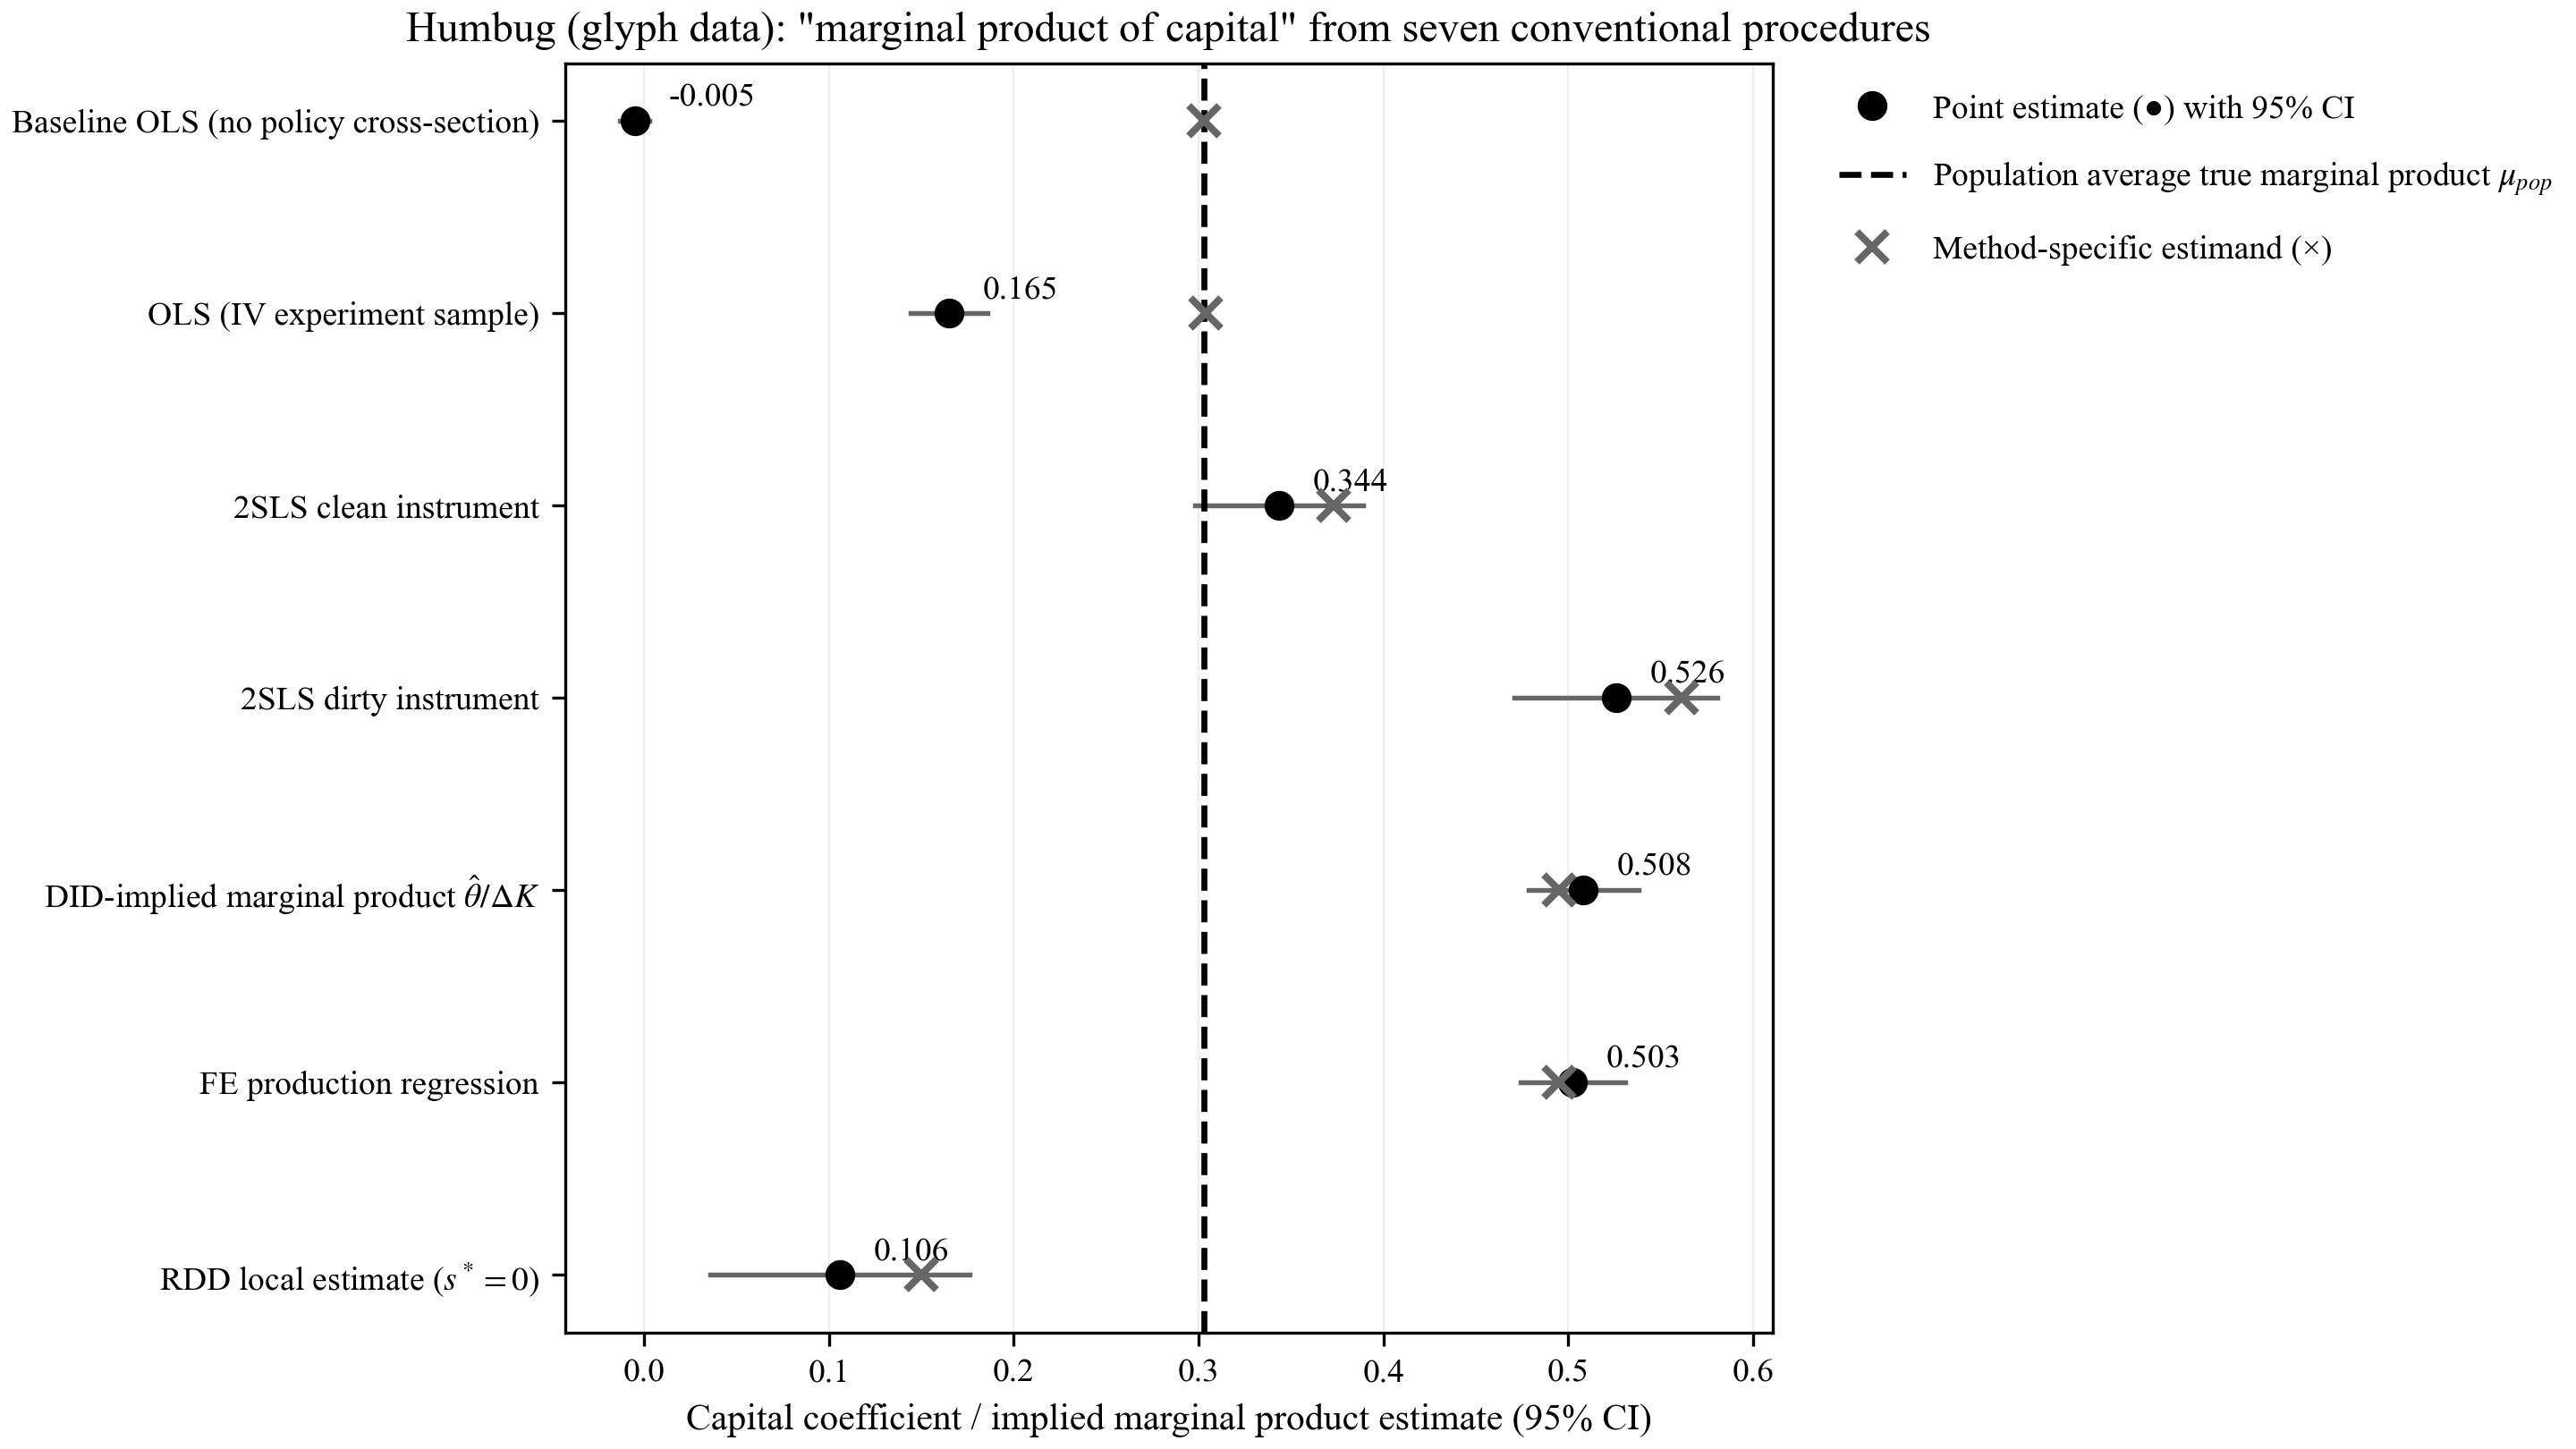
\includegraphics[width=0.92\textwidth]{fig6_answers.png}
\caption{HUMBUG 字形世界：七种常规程序给出的“资本边际产出”\\[1pt]\small The HUMBUG-glyph world: “marginal products of capital” from seven routine procedures}\label{fig:answers}
\end{figure}

图~\ref{fig:answers} 把 HUMBUG 世界的全部常规程序放在同一坐标下：基准 OLS（$-0.005$）、实验样本 OLS（0.165）、干净 2SLS（0.344）、脏 2SLS（0.526）、DID 隐含边际产出（0.508）、FE 生产回归（0.503）与 RDD 局部估计（0.106）。七个数字中没有一个等于总体平均真实边际产出 0.298，且它们彼此之间也互不相同。每个程序都在自己的意义上“正确”：诊断全部通过、系数全部显著、程序互相印证——但“资本边际产出”在这个世界根本没有定义，任何精确的数字都是对不存在之物的度量。

Figure~\ref{fig:answers} puts all routine procedures in the HUMBUG world on the same axis: baseline OLS ($-0.005$), experiment-sample OLS (0.165), clean 2SLS (0.344), dirty 2SLS (0.526), DID implied marginal product (0.508), FE production regression (0.503), and RDD local estimate (0.106). None of the seven equals the population-average true marginal product of 0.298, and they differ among themselves. Each procedure is “correct” in its own sense: all diagnostics pass, all coefficients are significant, procedures corroborate one another—but “the marginal product of capital” is undefined in this world, and any precise number is a measurement of something that does not exist.

\subsection[方法 $\times$ 识别对象 $\times$ 失败层次]{方法 $\times$ 识别对象 $\times$ 失败层次\\[1pt]\normalsize Method $\times$ estimand $\times$ failure layer}

\begin{table}[htbp]
\centering
\small
\caption{三种方法的识别对象与失败层次\\[1pt]\small Estimands and failure layers of the three methods}\label{tab:fail}
\begin{tabularx}{\textwidth}{L{0.16\textwidth} L{0.27\textwidth} Y L{0.19\textwidth}}
\toprule
\makecell[l]{方法\\Method} & \makecell[l]{识别对象（概率极限）\\Estimand (plim)} & \makecell[l]{为何不等于资本边际产出\\Why not the marginal product of capital} & \makecell[l]{失败层次\\Failure layer} \\
\midrule
\bip{基准 OLS}{Baseline OLS} & \bip{$\mathrm{Cov}(k,q)/\mathrm{Var}(k)$}{Cross-sectional covariance ratio} & \bip{字形世界无函数关系；实验样本中另有内生性}{No functional relation in the glyph world; additional endogeneity in the experiment sample} & \bip{不适用（描述性）}{Not applicable (descriptive)} \\
\bip{2SLS 干净}{2SLS clean} & \bip{$E[\mu\pi]/E[\pi]$}{Complier-weighted average} & \bip{依从者是受信贷约束、高边际产出的企业，不代表全体}{Compliers are credit-constrained, high-MPK firms; not representative of all firms} & \bip{解释鸿沟}{Interpretive gap} \\
\bip{2SLS 脏}{2SLS dirty} & \bip{$(E[\mu\pi]+\delta)/E[\pi]$}{Complier-weighted plus direct channel} & \bip{排除限制违背：直接渠道按 $1/E[\pi]$ 折入资本系数}{Exclusion violation: the direct channel enters at $1/E[\pi]$} & \bip{统计识别失败}{Statistical identification failure} \\
\bip{DID 隐含}{DID implied} & \bip{$E[\mu|\text{处理组}]+\varphi/\Delta k$}{Treated mean plus direct effect} & \bip{政策直接渠道（融资/技术/竞争）+ 处理组选择性}{Direct policy channels (financing/technology/competition) plus treatment selection} & \bip{识别失败 + 解释鸿沟}{Identification failure + interpretive gap} \\
\bip{RDD}{RDD} & \bip{$E[\mu|s{=}s^*]$}{Threshold local average} & \bip{异质性下局部参数随门槛移动，不可外推}{The local parameter moves with the threshold under heterogeneity; not extrapolable} & \bip{过度推论}{Over-extrapolation} \\
\bottomrule
\end{tabularx}
\end{table}

\subsection[对经验研究的含义]{对经验研究的含义\\[1pt]\normalsize Implications for empirical research}

从“识别出了某个资本相关因果效应”跳到“测得了资本的边际产出”，再跳到“总量生产函数得到证实”。对经验研究有三点具体含义：
\begin{enumerate}
  \item 报告识别策略时应同时报告识别对象——工具变量作用于哪些依从者、政策作用于哪些处理组、门槛截到了哪些企业；
  \item 存在异质性与直接渠道时，不同方法给出不同数字是常态而非异常，程序间的相互印证（如 DID 与 FE 回归一致）不能替代概念效度；
  \item 任何把局部因果效应外推为总量生产规律的做法（如用门槛附近的弹性预测总体政策效果），都应当显式承担本实验图~\ref{fig:rdd}(d) 所示的那类外推风险。
\end{enumerate}
Jumping from “a capital-related causal effect has been identified” to “the marginal product of capital has been measured,” and then to “the aggregate production function is confirmed,” involves three specific implications for empirical work: (i) when reporting an identification strategy, report the estimand as well—which compliers the instrument affects, which treated units the policy covers, which firms the threshold selects. (ii) with heterogeneity and direct channels, different methods yielding different numbers is the rule rather than the exception, and corroboration among procedures (e.g., DID agreeing with FE regression) is no substitute for conceptual validity. (iii) any attempt to extrapolate local causal effects to aggregate production laws (e.g., using a near-threshold elasticity to predict an economy-wide policy effect) should explicitly bear the kind of extrapolation risk shown in Figure~\ref{fig:rdd}(d).

\subsection[复现指南]{复现指南\\[1pt]\normalsize Replication guide}

全部交付文件位于 \texttt{humbug\_output} 目录：模拟脚本 \texttt{humbug\_iv\_did\_rdd.ipynb}（Anaconda 环境打开即用，代码分单元格、图表内联）、结果文件 \texttt{results.json}、逐次蒙特卡洛记录 \texttt{mc\_raw.csv}、汇总表 \texttt{MC汇总表.xlsx}、六张图（\texttt{figures} 子目录）与本说明文档。\texttt{-{}-modes humbug} 可只跑单一模式，\texttt{-{}-quick} 以 20 次蒙特卡洛快速自检。切换则修改 \texttt{CONFIG} 字典的 \texttt{mode} / \texttt{modes\_to\_run} / \texttt{focus\_mode} 字段。文档中全部表格数字由构建脚本运行时从 \texttt{results.json} 读取，与模拟输出严格一致。本文档为 LaTeX 源码，与 \texttt{figures} 目录同处一目录后，用 \texttt{xelatex} 连续编译两遍（或 \texttt{tectonic} 一遍）即得 PDF。

All deliverables live in the \texttt{humbug\_output} directory: the simulation script \texttt{humbug\_iv\_did\_rdd.ipynb} (ready to open in an Anaconda environment, with code split into cells and figures inline), the results file \texttt{results.json}, the per-replication Monte Carlo log \texttt{mc\_raw.csv}, the summary workbook \texttt{MC汇总表.xlsx}, the six figures (in the \texttt{figures} subdirectory), and this documentation. Use \texttt{-{}-modes humbug} to run a single mode; use \texttt{-{}-quick} for a 20-replication smoke test. To switch modes, edit the \texttt{mode}, \texttt{modes\_to\_run}, and \texttt{focus\_mode} fields of the \texttt{CONFIG} dictionary. All table numbers in this document are read at build time from \texttt{results.json} and match the simulation output exactly. This document is LaTeX source; place it alongside the \texttt{figures} directory and compile twice with \texttt{xelatex} (or once with \texttt{tectonic}) to obtain a PDF.

\appendix

\ctexset{section/name={附录}}

\section[关键代码]{关键代码（以 def 函数块为说明单元）\\[2pt]\normalsize Key code (by def function blocks)}

本附录以 def 函数块为最小代码说明单元，收录 HUMBUG 矢量生成、\texttt{CONFIG} 字典与三个实验的核心估计函数。正文中各实验的实现函数在 5—7 节均已按名引用。

This appendix uses def function blocks as the minimal unit of code exposition and collects the HUMBUG vector generation, the \texttt{CONFIG} dictionary, and the core estimation functions of the three experiments. The implementation functions of the experiments in the main text are referenced by name in Sections 5--7.

\subsection[CONFIG]{CONFIG：数据给定模式的切换开关\\[1pt]\normalsize CONFIG: the switch for data-generating modes}

全部数据生成与实验参数集中于此字典。\texttt{mode} 字段切换数据给定模式（\texttt{humbug} / \texttt{neoclassical} / \texttt{identity}）；\texttt{hetero} 子字典定义真实边际响应 $\mu$ 的异质性结构；\texttt{iv} / \texttt{did} / \texttt{rdd} 三个子字典分别对应三组实验；\texttt{mc\_reps} 为蒙特卡洛次数。

All data-generation and experiment parameters are centralized in this dictionary. The \texttt{mode} field switches the data-generating mode (\texttt{humbug} / \texttt{neoclassical} / \texttt{identity}); the \texttt{hetero} sub-dictionary defines the heterogeneity structure of the true marginal response $\mu$; the \texttt{iv}, \texttt{did}, and \texttt{rdd} sub-dictionaries correspond to the three experiments; \texttt{mc\_reps} sets the number of Monte Carlo replications.

\begin{lstlisting}[style=pycode]
CONFIG = {
    # —— 数据给定模式 ("humbug" | "neoclassical" | "identity") ——
    "mode": "humbug",                       # 当前聚焦模式 (切换数据给定方式)
    "modes_to_run": ["humbug", "neoclassical", "identity"],
    "focus_mode": "humbug",                 # 详细图表 (图2-4) 所用模式
    "seed": 2026,

    # —— HUMBUG 字形 ——
    "n_humbug_points": 2600,

    # —— 共同结构参数 ——
    "alpha": 0.30,                          # 真实平均资本弹性 / 恒等式斜率 r
    # μ_i 异质性 (仅 humbug 模式): μ = α + a_c·c + a_s·s + a_q·(s²-1) + e
    "hetero": {"a_c": 0.20, "a_s": -0.10, "a_q": 0.15, "sd_e": 0.05},

    # —— 实验一: IV ——
    "iv": {"n": 800, "pi_lo": 0.15, "pi_hi": 0.55, "pi_c": 0.9,
           "sd_v": 0.05, "sd_e": 0.02, "delta_dirty": 0.08},

    # —— 实验二: DID ——
    "did": {"n": 400, "T": 4, "post_start": 2, "dk": 0.25, "sd_nu": 0.04,
            "phi": 0.03, "tau": [0.000, 0.012, 0.024, 0.036], "sd_u": 0.02},

    # —— 实验三: RDD ——
    "rdd": {"n": 1200, "s_max": 3.0, "gamma": 0.30, "sd_w": 0.03, "sd_e": 0.02,
            "h": 1.0, "h_grid": [0.5, 1.0, 1.5, 2.0],
            "pseudo": [-2.0, -1.5, -1.0, -0.5, 0.0, 0.5, 1.0, 1.5, 2.0]},

    # —— 蒙特卡洛 ——
    "mc_reps": 500,

    # —— 输出 ——
    "out_dir": "/home/z/my-project/download/humbug_causal",
}
\end{lstlisting}

\subsection[HUMBUG]{HUMBUG(n\_total)：矢量字形数据生成\\[1pt]\normalsize HUMBUG(n\_total): vector-glyph data generation}

按矢量方式生成数据：\texttt{TextPath} 把“HUMBUG”渲染为衬线粗体轮廓多边形，逐段计算弧长并均匀采样，最后归一化到 $(k, q)$ 平面的设定范围。生成结果确定可复现，\texttt{get\_letters()} 对其做全局缓存。

Data are generated as vectors: \texttt{TextPath} renders “HUMBUG” as serif bold outline polygons, arc lengths are computed and sampled uniformly per segment, and the result is normalized to the specified range in the $(k,q)$ plane. The output is deterministic and reproducible; \texttt{get\_letters()} caches it globally.

\begin{lstlisting}[style=pycode]
def HUMBUG(n_total=2600):
    """用 matplotlib 矢量字形沿轮廓弧长均匀采样生成 HUMBUG 数据。

    返回 (x, y): (k, q) 平面上的 ~n_total 个点, x∈[2.05, 3.90], y∈[0.60, 0.82],
    在平面上拼出 "HUMBUG" 六个字母 (衬线粗体)。
    """
    fp = FontProperties(family="DejaVu Serif", weight="bold")
    tp = TextPath((0, 0), "HUMBUG", size=1.0, prop=fp)
    # 沿路径弧长均匀采样
    segs = []
    for poly in tp.to_polygons():
        poly = np.asarray(poly)
        d = np.sqrt(((poly[1:] - poly[:-1]) ** 2).sum(axis=1))
        segs.append((poly, np.concatenate([[0], np.cumsum(d)])))
    total_len = sum(s[1][-1] for s in segs)
    pts = []
    for poly, cum in segs:
        n = max(2, int(round(n_total * cum[-1] / total_len)))
        u = np.linspace(0, cum[-1], n)
        x = np.interp(u, cum, poly[:, 0])
        y = np.interp(u, cum, poly[:, 1])
        pts.append(np.column_stack([x, y]))
    P = np.concatenate(pts)
    # 归一化到 (k, q) 平面的合适范围
    x, y = P[:, 0], P[:, 1]
    x = 2.05 + 1.85 * (x - x.min()) / (x.max() - x.min())
    y = 0.60 + 0.22 * (y - y.min()) / (y.max() - y.min())
    return x, y
\end{lstlisting}

\subsection[make\_firms]{make\_firms(mode, n, rng)：三模式企业截面\\[1pt]\normalsize make\_firms(mode, n, rng): firm cross-sections in the three modes}

按 \texttt{mode} 生成 $n$ 家企业的初始 $(k_0, q_0)$ 与真实边际响应 $\mu$。humbug 模式从字形点集抽样并构造异质 $\mu$；neoclassical 与 identity 模式分别给出带噪声的真生产函数与精确成立的恒等式，$\mu$ 同质。

Generates the initial $(k_0,q_0)$ and true marginal response $\mu$ for $n$ firms according to \texttt{mode}. The humbug mode samples from the glyph set and constructs a heterogeneous $\mu$; the neoclassical and identity modes provide, respectively, a noisy genuine production function and an exactly satisfied identity, with homogeneous $\mu$.

\begin{lstlisting}[style=pycode]
def make_firms(mode, n, rng):
    """按数据给定模式抽取 n 家企业的初始截面 (k0, q0) 与真实边际响应 μ。

    - humbug      : 从 HUMBUG 字形点中抽取 (k0, q0); 不可观测异质性
                    c (信贷约束) 与 s (企业规模) 独立抽取;
                    μ = α + a_c·c + a_s·s + a_q·(s²-1) + e, E[μ]=α。
    - neoclassical: k0~N(2.9,0.35), q0 = -0.20 + α·k0 + ε (真生产函数);
                    μ_i = α 同质。
    - identity    : q0 = -0.20 + α·k0 精确成立 (会计恒等式, R²=1);
                    μ_i = α 同质 (恒等式斜率 = 利润率参数)。
    """
    if mode == "humbug":
        kx, qy = get_letters()
        idx = rng.choice(len(kx), size=n, replace=True)
        k0 = kx[idx] + rng.normal(0, 0.005, n)     # 微小抖动, 避免点完全重合
        q0 = qy[idx] + rng.normal(0, 0.005, n)
        h = CONFIG["hetero"]
        c = rng.normal(size=n)
        s = np.clip(rng.normal(size=n), -CONFIG["rdd"]["s_max"], CONFIG["rdd"]["s_max"])
        mu = (CONFIG["alpha"] + h["a_c"] * c + h["a_s"] * s
              + h["a_q"] * (s ** 2 - 1.0) + rng.normal(0, h["sd_e"], n))
    elif mode == "neoclassical":
        k0 = rng.normal(2.9, 0.35, n)
        q0 = -0.20 + CONFIG["alpha"] * k0 + rng.normal(0, 0.01, n)
        c = rng.normal(size=n)
        s = np.clip(rng.normal(size=n), -CONFIG["rdd"]["s_max"], CONFIG["rdd"]["s_max"])
        mu = np.full(n, CONFIG["alpha"])
    elif mode == "identity":
        k0 = rng.normal(2.9, 0.35, n)
        q0 = -0.20 + CONFIG["alpha"] * k0           # 恒等式精确成立, 无噪声
        c = rng.normal(size=n)
        s = np.clip(rng.normal(size=n), -CONFIG["rdd"]["s_max"], CONFIG["rdd"]["s_max"])
        mu = np.full(n, CONFIG["alpha"])
    else:
        raise ValueError("未知数据给定模式: %s" % mode)
    return {"k0": k0, "q0": q0, "mu": mu, "c": c, "s": s}
\end{lstlisting}

\subsection[iv\_estimate]{iv\_estimate(firms, shock, arm)：2SLS 与双重基准\\[1pt]\normalsize iv\_estimate(firms, shock, arm): 2SLS and dual benchmarks}

在给定冲击 $(Z, v, e, \pi)$ 下构造资本与产出，估计实验样本 OLS、第一阶段与恰好识别 2SLS（稳健方差由 \texttt{iv\_robust()} 提供），并同时计算模拟器视角的三重基准：总体平均 $\mu_{\mathrm{pop}}$、依从者加权平均 $E[\mu\pi]/E[\pi]$ 与含 $\delta$ 的识别对象。\texttt{arm} 参数切换干净/脏两臂。

Constructs capital and output under the given shocks $(Z,v,e,\pi)$, estimates the experiment-sample OLS, the first stage, and the just-identified 2SLS (robust variance from \texttt{iv\_robust()}), and simultaneously computes three benchmarks from the simulator's perspective: the population mean $\mu_{\mathrm{pop}}$, the complier-weighted average $E[\mu\pi]/E[\pi]$, and the $\delta$-inclusive estimand. The \texttt{arm} argument switches clean vs.\ dirty.

\begin{lstlisting}[style=pycode]
def iv_estimate(firms, shock, arm):
    """在给定冲击下估计 OLS 与 2SLS, 并计算模拟器视角的三重基准。

    恰好识别 2SLS 的概率极限 (Wald 估计量):
        clean: β → E[μπ]/E[π]  (依从者加权平均, LATE 型参数)
        dirty: β → (E[μπ] + δ)/E[π]  (混入直接渠道, 排除限制被违背)
    两面都不等于总体平均 μ_pop = E[μ] —— 这就是"因果参数与理论概念的解释鸿沟"。
    """
    iv = CONFIG["iv"]
    Z, v, e, pi = shock["Z"], shock["v"], shock["e"], shock["pi"]
    dk = pi * Z + v
    k = firms["k0"] + dk
    delta = iv["delta_dirty"] if arm == "dirty" else 0.0
    q = firms["q0"] + firms["mu"] * dk + delta * Z + e

    one = np.ones_like(k)
    m_ols = ols(q, np.column_stack([one, k]))
    fs = ols(k, np.column_stack([one, Z]))
    F = float(fs["t"][1] ** 2)
    beta, se, _ = iv_robust(q, np.column_stack([one, k]),
                            np.column_stack([one, Z]))

    mu = firms["mu"]
    n = len(mu)
    mu_pop = float(mu.mean())
    mu_comp = float((mu * pi).sum() / pi.sum())
    estimand = float(((mu * pi).sum() / n + delta) / (pi.sum() / n))
    return {
        "arm": arm, "delta": delta,
        "pi_hat": float(fs["beta"][1]), "pi_se": float(fs["se"][1]),
        "first_stage_F": F,
        "ols_beta": float(m_ols["beta"][1]), "ols_se": float(m_ols["se"][1]),
        "beta": float(beta[1]), "se": float(se[1]),
        "mu_pop": mu_pop, "mu_compliers": mu_comp, "estimand": estimand,
        "n": n,
    }
\end{lstlisting}

\subsection[did\_estimate]{did\_estimate(panel)：TWFE、隐含边际产出与基准\\[1pt]\normalsize did\_estimate(panel): TWFE, implied MPK, and benchmarks}

对 \texttt{did\_simulate()} 生成的面板做双向固定效应变换（\texttt{twoway\_demean()}），估计政策总效应 $\theta$、资本的 DID 增量 $\Delta K$、隐含边际产出 $\theta/\Delta K$ 与 FE 生产回归，并计算处理组真实平均、识别对象与 $\mu_{\mathrm{pop}}$。安慰剂版本见 \texttt{did\_placebo()}。

Applies the two-way fixed-effects transformation (\texttt{twoway\_demean()}) to the panel generated by \texttt{did\_simulate()}, estimating the overall policy effect $\theta$, the DID capital increment $\Delta K$, the implied marginal product $\theta/\Delta K$, and the FE production regression, and computing the treated-group true mean, the estimand, and $\mu_{\mathrm{pop}}$. The placebo version is \texttt{did\_placebo()}.

\begin{lstlisting}[style=pycode]
def did_estimate(panel):
    """TWFE 双重差分: ATT (θ)、资本 DID (ΔK)、隐含边际产出 (θ/ΔK) 与 FE 生产回归。

    DID 识别的是政策总效应: θ = E[μ|Treat]·Δk + φ;
    研究者若以 θ/ΔK 解读为"资本边际产出", 得到 E[μ|Treat] + φ/Δk,
    既非总体平均 μ_pop, 也非处理组真实平均 —— 识别成功 ≠ 理论概念。
    """
    d = CONFIG["did"]
    k, q, D = panel["k"], panel["q"], panel["D"]
    n, T = panel["n"], panel["T"]
    qd = twoway_demean(q).ravel()
    Dd = twoway_demean(D).ravel()
    kd = twoway_demean(k).ravel()

    sxx = float((Dd * Dd).sum())
    theta = float((qd * Dd).sum() / sxx)
    resid = qd - theta * Dd
    dof = n * T - n - T
    s2 = float(resid @ resid) / dof
    se_theta = math.sqrt(s2 / sxx)

    sxxk = float((kd * kd).sum())
    fe = float((qd * kd).sum() / sxxk)
    residk = qd - fe * kd
    se_fe = math.sqrt(float(residk @ residk) / dof / sxxk)

    tr, po = panel["treat"], panel["post"]
    dk_did = ((k[tr][:, po].mean() - k[tr][:, ~po].mean())
              - (k[~tr][:, po].mean() - k[~tr][:, ~po].mean()))

    mu_treated = float(panel["mu"][tr].mean())
    implied_true = mu_treated + d["phi"] / d["dk"]
    return {
        "theta": theta, "se_theta": se_theta,
        "dk_did": float(dk_did),
        "implied": theta / dk_did,
        "implied_se": se_theta / dk_did,
        "fe": fe, "se_fe": se_fe,
        "mu_treated": mu_treated, "implied_true": implied_true,
        "mu_pop": float(panel["mu"].mean()),
        "share_treated": float(tr.mean()), "n": n, "T": T,
    }
\end{lstlisting}

\subsection[rdd\_estimate]{rdd\_estimate(data, h)：局部线性模糊 RDD\\[1pt]\normalsize rdd\_estimate(data, h): local-linear fuzzy RDD}

在 $|s - s^*| \le h$ 窗口内以门槛指示 $D$ 作资本的工具做局部 2SLS（两侧斜率允许不同），$\hat{\beta}$ 恒等于两侧局部线性跳跃之比 $J_q/J_k$；同时报告 $J_k$、$J_q$ 与窗口样本量。伪门槛扫描与带宽敏感性均复用本函数。

Runs a local 2SLS within the window $|s-s^*|\le h$, using the threshold indicator $D$ as an instrument for capital (slopes allowed to differ across sides); $\hat\beta$ is identically the ratio of the two local-linear jumps $J_q/J_k$; it also reports $J_k$, $J_q$, and the window sample size. Both the pseudo-threshold scan and the bandwidth sensitivity reuse this function.

\begin{lstlisting}[style=pycode]
def rdd_estimate(data, h):
    """模糊 RDD 局部线性 2SLS: 窗口 |s-c|≤h 内, 用 D 作 k 的工具。

    估计方程 (两侧斜率允许不同):
      q = β·k + a + b_l·(s-c)·(1-D) + b_r·(s-c)·D + 误差
      工具: [1, (s-c)(1-D), (s-c)D, D]
    β̂ 恒等于两侧局部线性跳跃之比 J_q/J_k, 概率极限为 E[μ|s=c]。
    """
    s, k, q, D = data["s"], data["k"], data["q"], data["D"]
    c = data["cutoff"]
    m = np.abs(s - c) <= h
    nw = int(m.sum())
    sc = s[m] - c
    Dm = D[m]
    one = np.ones(nw)
    exog = np.column_stack([one, sc * (1.0 - Dm), sc * Dm])
    X = np.column_stack([exog, k[m]])
    Z = np.column_stack([exog, Dm])
    beta, se, _ = iv_robust(q[m], X, Z)
    fsk = ols(k[m], np.column_stack([exog, Dm]))
    rfq = ols(q[m], np.column_stack([exog, Dm]))
    return {"beta": float(beta[3]), "se": float(se[3]),
            "Jk": float(fsk["beta"][3]), "Jq": float(rfq["beta"][3]),
            "n_win": nw, "h": h}
\end{lstlisting}

\subsection[run\_mc]{run\_mc(mode, reps)：蒙特卡洛主循环\\[1pt]\normalsize run\_mc(mode, reps): Monte Carlo main loop}

重复 \texttt{reps} 次单次实验（\texttt{mc\_one()}：重抽企业与全部冲击、跑全部估计量），对每个估计量汇总均值、标准差、分位数、相对 $\mu_{\mathrm{pop}}$ 与相对自身识别对象的双重偏差、以及对 $\mu_{\mathrm{pop}}$ 的 95\% 置信区间覆盖率。

Repeats the single-run experiment \texttt{reps} times (\texttt{mc\_one()}: redraws firms and all shocks and runs every estimator), and for each estimator summarizes the mean, standard deviation, quantiles, dual biases relative to $\mu_{\mathrm{pop}}$ and to its own estimand, and 95\% CI coverage of $\mu_{\mathrm{pop}}$.

\begin{lstlisting}[style=pycode]
def run_mc(mode, reps):
    """蒙特卡洛主循环: reps 次重复 → 每个估计量的分布与双重偏差汇总。"""
    rows = [mc_one(mode, rep) for rep in range(reps)]

    def arr(key):
        return np.array([row[key] for row in rows], float)

    mu_pop = arr("mu_pop").mean()
    estimators = {
        "ols_base": {"est": "ols_base", "se": "ols_base_se", "estimand": "mu_pop"},
        "iv_clean": {"est": "iv_clean", "se": "iv_clean_se", "estimand": "mu_comp"},
        "iv_dirty": {"est": "iv_dirty", "se": "iv_dirty_se", "estimand": "ivd_estimand"},
        "did_implied": {"est": "did_implied", "se": "did_implied_se", "estimand": "did_implied_true"},
        "did_fe": {"est": "did_fe", "se": "did_fe_se", "estimand": "did_implied_true"},
        "rdd": {"est": "rdd", "se": "rdd_se", "estimand": "rdd_local_true"},
    }
    summary = {}
    for name, spec in estimators.items():
        est = arr(spec["est"])
        estand = arr(spec["estimand"]).mean()
        item = {
            "mean": float(est.mean()), "sd": float(est.std(ddof=1)),
            "q025": float(np.percentile(est, 2.5)),
            "q975": float(np.percentile(est, 97.5)),
            "estimand": float(estand),
            "bias_vs_pop": float(est.mean() - mu_pop),
            "bias_vs_estimand": float(est.mean() - estand),
        }
        if spec["se"] is not None:
            se = arr(spec["se"])
            item["cover_pop"] = float(np.mean(np.abs(est - mu_pop) <= 1.96 * se))
        else:
            item["cover_pop"] = None
        summary[name] = item
    summary["_meta"] = {
        "reps": reps, "mu_pop": float(mu_pop),
        "mu_comp": float(arr("mu_comp").mean()),
        "ivd_estimand": float(arr("ivd_estimand").mean()),
        "did_treated_mu": float(arr("did_treated_mu").mean()),
        "did_implied_true": float(arr("did_implied_true").mean()),
        "rdd_local_true": float(arr("rdd_local_true").mean()),
        "iv_F_min": float(arr("iv_F").min()), "iv_F_med": float(np.median(arr("iv_F"))),
        "did_placebo_mean": float(arr("did_placebo").mean()),
        "did_placebo_cover0": float(np.mean(
            np.abs(arr("did_placebo")) <= 1.96 * arr("did_placebo_se"))),
        "rdd_h05_mean": float(arr("rdd_h05").mean()),
        "rdd_h15_mean": float(arr("rdd_h15").mean()),
        "rdd_h20_mean": float(arr("rdd_h20").mean()),
    }
    return summary, rows
\end{lstlisting}

\section[参数表与交付文件清单]{参数表与交付文件清单\\[2pt]\normalsize Parameter table and deliverables checklist}

\begin{table}[htbp]
\centering
\small
\caption{主要参数（\texttt{CONFIG} 节选）\\[1pt]\small Main parameters (excerpt of \texttt{CONFIG})}\label{tab:params}
\begin{tabularx}{\textwidth}{L{0.22\textwidth} L{0.34\textwidth} Y}
\toprule
\makecell[l]{参数\\Parameter} & \makecell[l]{取值\\Value} & \makecell[l]{含义\\Meaning} \\
\midrule
\texttt{alpha} & 0.30 & \bip{真实平均资本弹性 / 恒等式斜率}{True average capital elasticity / identity slope} \\
\texttt{hetero} & $a_c=0.20$, $a_s=-0.10$, $a_q=0.15$, sd$_e=0.05$ & \bip{$\mu=\alpha+a_c c+a_s s+a_q(s^2-1)+e$（仅 humbug 模式）}{Heterogeneous $\mu$ (humbug mode only)} \\
\texttt{iv.n} / \texttt{delta\_dirty} & 800 / 0.08 & \bip{IV 样本量 / 脏工具直接渠道强度}{IV sample size / dirty-instrument direct-channel strength} \\
\texttt{iv.pi} & $0.15+0.55\Phi(0.9c)$ & \bip{依从强度（恒正、单调）}{Compliance (positive, monotone)} \\
\texttt{did.n} / \texttt{T} / \texttt{dk} / \texttt{phi} & 400 / 4 / 0.25 / 0.03 & \bip{企业数 / 期数 / 补贴资本增量 / 政策直接效应}{Firms / periods / subsidy capital increment / direct policy effect} \\
\texttt{rdd.n} / \texttt{gamma} / \texttt{h} & 1200 / 0.3 / 1.0 & \bip{样本量 / 门槛资本跳升 / 带宽}{Sample size / threshold capital jump / bandwidth} \\
\texttt{mc\_reps} / \texttt{seed} & 500 / 2026 & \bip{蒙特卡洛次数 / 随机种子}{MC replications / seed} \\
\bottomrule
\end{tabularx}
\end{table}

\begin{table}[htbp]
\centering
\small
\caption{交付文件清单\\[1pt]\small Deliverables checklist}\label{tab:files}
\begin{tabularx}{\textwidth}{L{0.38\textwidth} Y}
\toprule
\makecell[l]{文件\\File} & \makecell[l]{内容\\Contents} \\
\midrule
\path{humbug_iv_did_rdd.ipynb} & \bip{Jupyter Notebook 环境的脚本（代码分单元格、图表内联、pandas 汇总、Excel 导出）}{Notebook script (code in cells, inline figures, pandas summary, Excel export)} \\
\path{results.json} & \bip{全部单次结果与蒙特卡洛汇总（本文档数字的来源）}{All single-run results and MC summaries (source of the numbers in this document)} \\
\path{mc_raw.csv} & \bip{500 $\times$ 3 模式的逐次估计原始记录}{Raw per-replication records, 500 $\times$ 3 modes} \\
\path{MC_notebook.xlsx} & \bip{MC 汇总 / 单次结果 / 参数三个工作表}{Three worksheets: MC summary / single runs / parameters} \\
\texttt{fig1}–\texttt{fig6}\texttt{.png} & \bip{六张灰阶图表（200 dpi）}{Six grayscale figures (200 dpi)} \\
\path{readme.tex} & \bip{本文档（LaTeX 源码；xelatex 两遍或 tectonic 一遍编译）}{This document (LaTeX source; compile twice with xelatex or once with tectonic)} \\
\bottomrule
\end{tabularx}
\end{table}

\section*{参考文献 References}

\addcontentsline{toc}{section}{参考文献 References}

{\footnotesize\noindent\hangindent 2em\hangafter 1 Angrist, J. D., and J.-S. Pischke. 2009. \emph{Mostly Harmless Econometrics: An Empiricist's Companion}. Princeton: Princeton University Press.\par}

{\footnotesize\noindent\hangindent 2em\hangafter 1 Bertrand, M., E. Duflo, and S. Mullainathan. 2004. How Much Should We Trust Differences-in-Differences Estimates? \emph{Quarterly Journal of Economics}, 119(1): 249–275.\par}

{\footnotesize\noindent\hangindent 2em\hangafter 1 Cohen, A. J., and G. C. Harcourt. 2003. Whatever Happened to the Cambridge Capital Theory Controversies? \emph{Journal of Economic Literature}, 41(4): 1446–1465.\par}

{\footnotesize\noindent\hangindent 2em\hangafter 1 Felipe, J., and J. S. L. McCombie. 2013. \emph{The Aggregate Production Function and the Measurement of Technical Change: “Not Even Wrong.”} Cheltenham: Edward Elgar.\par}

{\footnotesize\noindent\hangindent 2em\hangafter 1 Imbens, G. W., and J. D. Angrist. 1994. Identification and Estimation of Local Average Treatment Effects. \emph{Econometrica}, 62(2): 467–475.\par}

{\footnotesize\noindent\hangindent 2em\hangafter 1 Lee, D. S., and T. Lemieux. 2010. Regression Discontinuity Designs in Economics. \emph{Journal of Economic Literature}, 48(2): 281–355.\par}

{\footnotesize\noindent\hangindent 2em\hangafter 1 Shaikh, A. 1974. Laws of Production and Laws of Algebra: The Humbug Production Function. \emph{Review of Economics and Statistics}, 56(1): 115–120.\par}

{\footnotesize\noindent\hangindent 2em\hangafter 1 Solow, R. M. 1957. Technical Change and the Aggregate Production Function. \emph{Review of Economics and Statistics}, 39(3): 312–320.\par}

\end{document}